\chapter{Case Study: The University of Brasília Herbarium (UB)}\label{casestudy_ub}
% herbarium page: http://florescer.unb.br/bol/

% -----
% Intro

In this chapter, we use the network models proposed in Chapter~\ref{chapter:network_models} to understand aspects regarding the taxonomic preferences and the collecting behavior of collectors who have contributed to the University of Brasília Herbarium with specimens records.
By exploring basic topological features of the networks, we investigate the formation of
(\textit{i}) groups of collectors with similar taxonomic interests;
(\textit{ii}) groups of taxa which are often recorded by similar sets of collectors; and
(\textit{iii}) groups of collectors who collaborate by recording specimens together in collecting expeditions. 
From the resulting network structure, we also identify collectors who are the most relevant for the herbarium, and how they contribute for the representativeness of each taxonomic group in the collection.
Taxa that are either widely collected or collected by very specific groups of collectors are also easily identified from the network structure.

The University of Brasília Herbarium (UB) is a reference collection for the flora of the Cerrado biome, being noticeably representative for families \textit{Cyperaceae}, \textit{Myrtaceae}, and \textit{Fabaceae}; as well as for cryptogams~(algae, mosses, and lichens).
%
The herbarium is physically located at the Biology Department of the University of Brasília (UnB-IB) since its foundation in 1963.
Table \ref{table:ub_collectors_florescer} lists some historically relevant collectors who have intensively contributed to the herbarium, according to the \textit{Florescer} project \cite{florescer}.

\art{Pedro, ha algo de estranho na Tabela 3... George Eiten nao tem anos de atividade; entre JAmes e Joseph ha uma linha sem nome; Xavantina-Cachimbo expedition nao seria um ``coletor''??? Enfim, veriica a tabela.}
\ped{Na tabela original, do projeto Florescer, não tem informação sobre período de atividades do George Eiten (embora eu tenha esta informação a partir das redes, mas ainda n as apresentei no texto). No caso do gap entre James e Joseph, é pq a linha abaixo do James ainda se refere a ele (um outro período de atividades). Como é a melhor maneira de representar isso?}

\begin{table}[H]
  \caption{Historically important collectors for the University of Brasília Herbarium~(UB).}
  \footnotesize
  \begin{center}
  \begin{tabular}{l l l}
      & Activity years & Contribution\\
      \hline
      William R. Anderson & 1962-1976 & Central Brazil Expedition (NYBG)\\
      Howard S. Irwin & 1962-1976 & Central Brazil Expedition (NYBG)\\
      George Eiten & \multicolumn{1}{c}{---} & Cerrado biome, mainly in MA state \\
      James Alexander Ratter & 
      	\begin{tabular}[t]{{@{}l@{}}}1968-1976 \\ 1996-2006\end{tabular} &
        \begin{tabular}[t]{{@{}l@{}}}Xavantina-Cachimbo expedition \\ Cerrado biome\end{tabular} \\
      Joseph Harold Kirkbride Junior & 1976-1983 & Flora of DF state\\
      Ana Lúcia Tostes Leite & 1982-1984 & Continental algae of DF state\\
      Carolyn Elinores Barnes Proença & 1981-current & Cerrado biome \\
      Maria das Graças Machado de Souza & 1982-current & Continental algae of DF and GO states\\
      \hline
  \end{tabular}
  \\[1.5em]
  \hfill Source: Florescer Project (\url{http://www.florescer.unb.br})
  %[\getrefnumber{footnote:florescer}]
  \end{center}
  \label{table:ub_collectors_florescer}
  \normalsize
\end{table}

%\footnote{\label{footnote:florescer} \url{http://florescer.unb.br/janela4.html}}.

In this case study, we have used the entire digitized collection of records from the UB herbarium \cite{gbif_ubdataset}, which is publicly available for download through the Global Biodiversity Information Facility (GBIF) data portal \cite{gbif}. 
After downloading the entire dataset through the portal, we first performed a quick exploratory analysis, for a general overview on its taxonomic composition, the temporal and geographical distribution of the records, as well as the main issues associated with the dataset~(Section~\ref{section:ub_exploration}).
We have also performed data cleaning and transformation routines for atomizing and mapping variants of collectors' names, improving the quality of data from which the network models are constructed~(Section \ref{section:ub_data_preparation}).
Finally, in Sections~\ref{section:ub_scn} and~\ref{section:ub_cwn}, we present the SCN and CWN models built from the UB dataset and explore some of their topological features. 
%
We have used the \textit{Python v.3.6} language loaded with packages \textit{Pandas}, \textit{Numpy}, and \textit{Matplotlib} for exploring the occurrence dataset; and the \textit{Caryocar} package (designed and implemented by us, in the context of this dissertation) for programatically constructing the SCN and CWN models from occurrence data.

% -------------------------------
% -------------------------------
% UB Dataset Exploratory Analysis

\section{Dataset exploration}\label{section:ub_exploration}
% Check {Haripersaud2009}

At the time of this study, the entire occurrences dataset from the UB herbarium had a total of $185311$ records and $235$ fields.
For our application, however, only a small subset of those fields were considered to be relevant and were thus included in our exploratory analysis.
Most of these fields (except for \textit{issue}), which we briefly describe below, follow \textit{Darwin Core} terms standards.\footnote{\url{http://rs.tdwg.org/dwc/terms}} The relevant fields we take into account in this work are:

% Terms definitions
\begin{description}[align=left,labelindent=1cm]
\item [recordedBy.] A string containing names of people or groups who have authored an occurrence record, separated by some delimiter character.
Although the vertical bar (` | ') bar is officially recommended by \textit{TDWG}, names are separated by a semicolon character (` ; ') in the UB dataset. 
The UB convention for collector names makes each of them composed of two parts, separated by a comma (` , ').
The first part is the collector's last name, with the first character capitalized; and the second part corresponds to the first initials of the names, all capitalized and appended with a period.
A collector named `\textit{João da Silva Simão}', for instance, would be included as `\textit{Simão, J. S.}'.
%
\item [eventDate.] A date-time string representing the moment when the recording act happened.
%
\item [stateProvince.] The name of the state where the occurrence was recorded.

\item [countryCode.] The code of the country where the occurrence was recorded.

\item [decimalLatitude.] The geographic latitude coordinate of the place where the occurrence was recorded. 
Datum is assumed to be \textit{WGS84} for all records in the UB herbarium.

\item [decimalLongitude.] The geographic longitude coordinate of the place where the occurrence was recorded.
Datum is assumed to be \textit{WGS84} for all records in the UB herbarium.

\item [issue.] A sequence of data issues that have been identified in the record.
This field is included by GBIF during data preprocessing, and is not part of the \textit{Darwin Core} standard.% https://www.gbif.org/infrastructure/processing

\item [scientificName.] The scientific name assigned to the specimen, at the lowest taxonomic resolution as it can be determined. The authorship of the name is also included for many records, although not relevant for this study.

\item [taxonRank.] The taxonomic rank of the name in the \textit{scientificName} field.
\end{description}

% --------------------------
% Taxonomic characterization
\paragraph*{Taxonomic composition.}
% 
For exploring the taxonomic composition of the dataset we first removed $10$ records with missing values for the \textit{scientificName} field.
From the remaining $185301$ records, most had a taxonomic resolution at the \textit{species} level ($75.96\%$), followed by \textit{genus} ($13.17\%$), and \textit{variety}($4.82\%$), as shown by absolute metrics in Table~\ref{table:dset_taxonomicres_counts}. 
However, the percentage of records which can be determined at the rank of \textit{species} is slightly higher ($82.23\%$), and is given by the cumulative metrics in the table. 
This happens because the \textit{species} identity of records at higher taxonomic resolutions (in this case \textit{form}, \textit{variety} and \textit{subspecies}) are directly determined, as explained in section \ref{section:biodiversity_terms}.
Similarly, although only $1.08\%$ of the records have the taxonomic resolution at the \textit{kingdom} level, all records are determined at that rank.

\begin{table}
  \caption[Number of records with taxonomic resolution at each rank.]{Number of records with taxonomic resolution at each rank. Ranks are ordered hierarchically, being \textit{FORM} the most restrictive (higher resolution) and \textit{KINGDOM} the broader (lower resolution) one. Absolute metrics show the number and percentage of records at each taxonomic resolution, while cumulative metrics show the number and percentage of records that are taxonomically determined at each rank.}
  \begin{center}
  \begin{tabular}{l r r r r}
       & count & \% & cumulative count & cumulative \% \\
      \hline
      FORM & 1000 & 0.5397 & 1000 & 0.5397\\
      VARIETY & 8935 & 4.8219 & 9935 & 5.3615\\
      SUBSPECIES & 1681 & 0.9072 & 11616 & 6.2687\\
      SPECIES & 140763 & 75.9645 & 152379 & 82.2332\\
      GENUS & 24397 & 13.1661 & 176776 & 95.3994\\
      FAMILY & 6223 & 3.3583 & 182999 & 98.7577\\
      PHYLUM & 294 & 0.1587 & 183293 & 98.9164\\
      KINGDOM & 2008 & 1.0836 & 185301 & 100.0000\\
      \hline
      Total & 185301 & 100.0000 & &
  \end{tabular}
  \end{center}
  \label{table:dset_taxonomicres_counts}
\end{table}

\luiz{parei a revisão aqui} 


Table \ref{table:taxa_counts} shows the number of distinct taxa at each rank and lists those with the highest amounts of records.
The herbarium is mostly composed of plants~(kingdom \textit{Plantae}, representing $96.72\%$ of the records), followed by \textit{Chromista}~(including some phyla of algae), \textit{Funghi}, and \textit{Bacteria}.
Vascular plants~(phylum \textit{Tracheophyta}) compose $82.89\%$ of the herbarium, although \textit{Bryohpyta} (mosses), \textit{Ochrophyta} (algae from kingdom \textit{Chromista}) and \textit{Charophtya} (algae from kingdom \textit{Plantae}) are also representative.
At the family rank, \textit{Fabaceae}, is the most representative one ($10.39\%$), followed by \textit{Myrtaceae} ($6.93\%$), \textit{Asteraceae} ($6.08\%$) and \textit{Rubiaceae} ($5.10\%$). 
The most collected species are \textit{Myrcia splendens}, \textit{Myrcia guianensis}, \textit{Eugenia punicifolia}, and \textit{Sematophyllum subpinnatum}, the first three flowering plants and the latter a species of moss.

\begin{table}[t]
  \caption[Number of distinct taxa at each taxonomic rank in the dataset.]{Number of distinct taxa at each taxonomic rank in the dataset. For each rank a list with its top-4 most recorded taxa is included with their respective counts.}
\begin{center}
  \begin{tabular}{c c c c c}
    & num of taxa & top-4 taxa & num of records & \% of records \\
   \hline
    kingdom & 5 &
	\begin{tabular}[t]{{@{}c@{}}}Plantae\\Chromista\\Fungi\\Bacteria\end{tabular} &
	\begin{tabular}[t]{{@{}r@{}}}179218\\4204\\1391\\342\end{tabular} &
	\begin{tabular}[t]{{@{}r@{}}}96.72\\2.27\\0.75\\0.18\end{tabular} \\ \\
    phylum & 12 &
	\begin{tabular}[t]{{@{}c@{}}}Tracheophyta\\Bryophyta\\Ochrophyta\\Charophyta\end{tabular} &
	\begin{tabular}[t]{{@{}r@{}}}153589\\16485\\4133\\3500\end{tabular} &
	\begin{tabular}[t]{{@{}r@{}}}82.89\\8.90\\2.23\\1.89\end{tabular} \\ \\
    class & 29 &
	\begin{tabular}[t]{{@{}c@{}}}Magnoliopsida\\Liliopsida\\Bryopsida\\Bacillariophyceae\end{tabular} &
	\begin{tabular}[t]{{@{}r@{}}}126288\\23004\\15899\\4133\end{tabular} &
	\begin{tabular}[t]{{@{}r@{}}}68.15\\12.41\\8.58\\2.23\end{tabular} \\ \\
    order & 136 &
	\begin{tabular}[t]{{@{}c@{}}}Myrtales\\Fabales\\Poales\\Malpighiales\end{tabular} &
	\begin{tabular}[t]{{@{}r@{}}}24312\\20846\\17159\\16188\end{tabular} &
	\begin{tabular}[t]{{@{}r@{}}}13.12\\11.25\\9.26\\8.74\end{tabular} \\ \\
    family & 507 &
	\begin{tabular}[t]{{@{}c@{}}}Fabaceae\\Myrtaceae\\Asteraceae\\Rubiaceae\end{tabular} &
	\begin{tabular}[t]{{@{}r@{}}}19254\\12833\\11271\\9447\end{tabular} &
	\begin{tabular}[t]{{@{}r@{}}}10.39\\6.93\\6.08\\5.10\end{tabular} \\ \\
    genus & 3374 &
	\begin{tabular}[t]{{@{}c@{}}}Myrcia\\Eugenia\\Mimosa\\Miconia\end{tabular} &
	\begin{tabular}[t]{{@{}r@{}}}4654\\3750\\2992\\2402\end{tabular} &
	\begin{tabular}[t]{{@{}r@{}}}2.51\\2.02\\1.61\\1.30\end{tabular} \\ \\
    species & 15379 &
	\begin{tabular}[t]{{@{}c@{}}}Myrcia splendens\\Myrcia guianensis\\Eugenia punicifolia\\Sematophyllum subpinnatum\end{tabular} &
	\begin{tabular}[t]{{@{}r@{}}}696\\560\\462\\438\end{tabular} &
	\begin{tabular}[t]{{@{}r@{}}}0.38\\0.30\\0.25\\0.24\end{tabular} \\      
  \hline
  \end{tabular}
\end{center}
  \label{table:taxa_counts}
\end{table}

\clearpage
% --------------------------
% Geographic characterization
\paragraph*{Geographic distribution.}

We then explored the geographic distribution of the herbarium records.
From the set of $185,301$ records, approximately $48\%$ (a total of $89,216$) were interpreted and tagged as having geospatial issues during internal preprocessing routines in the \textit{GBIF} platform~\cite{gbif_dataprocessing}.
Routines perform geospatial validation by checking, for each record: (\textit{i})~if geographical coordinates are erroneously assigned to zero latitude and longitude; (\textit{ii})~if geographic coordinates are in fact placed within the boundaries of the country, if the country is indicated; and (\textit{iii})~if the lat/long values are likely to having been accidentally swapped or negated during recording.
If inconsistencies are detected during the execution of such routines, issues are registered for each record, priorly to making the dataset available for download or query via an API. 
% http://www-old.gbif.org/infrastructure/processing

As shown in Figure \ref{fig:venn_geospatial_issues}, most geospatial issues are due to records being assigned to zero coordinates (zero latitude and longitude), which also makes them laying outside the country boundaries. 
As a consequence, they are tagged as having both the ``Zero Coordinates'' (ZC) and ``Country Coordinates Mismatch'' (CCM) issues, being represented in the Figure~\ref{fig:venn_geospatial_issues} as the intersection between CCM and ZC.
Some records with only the CCM issue were not misplaced in coordinates $(0,0)$, but were still improperly placed outside country frontiers. 
On the other hand, records with only the ZC issue are those which were misplaced in coordinates $(0,0)$, but were lacking information about the country, and therefore couldn't be classified as being outside the country frontiers.
Records that were not interpreted as having geospatial issues comprise approximately $52\%$ of the dataset, and the coordinates of those records that are located around the Brazilian territory are shown in Figure~\ref{fig:occurrence_map}. 

  \begin{figure}[ht]
  	\centering
    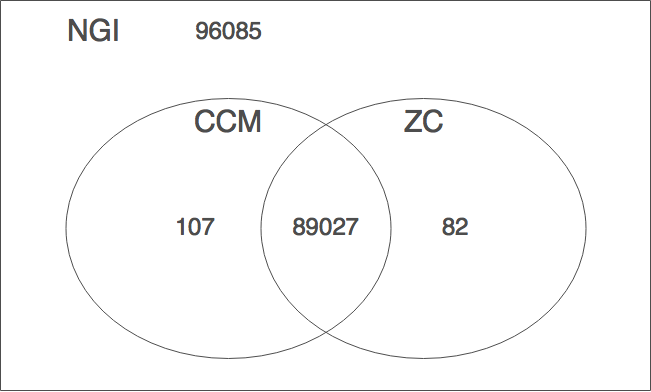
\includegraphics[width=0.6\linewidth]{figures/venn_geospatial_issues.png}
    \caption[Number of occurrences from the UB herbarium dataset classified within each geospatial issue class.]{Number of occurrences from the UB herbarium dataset classified within each geospatial issue class. \textit{NGI}: Records with no geospatial issues; \textit{CCM}: Country Coordinates Mismatch issue; \textit{ZC}: Zero Coordinates issue.}
    \label{fig:venn_geospatial_issues}
  \end{figure}


\begin{figure}[t]
\centering
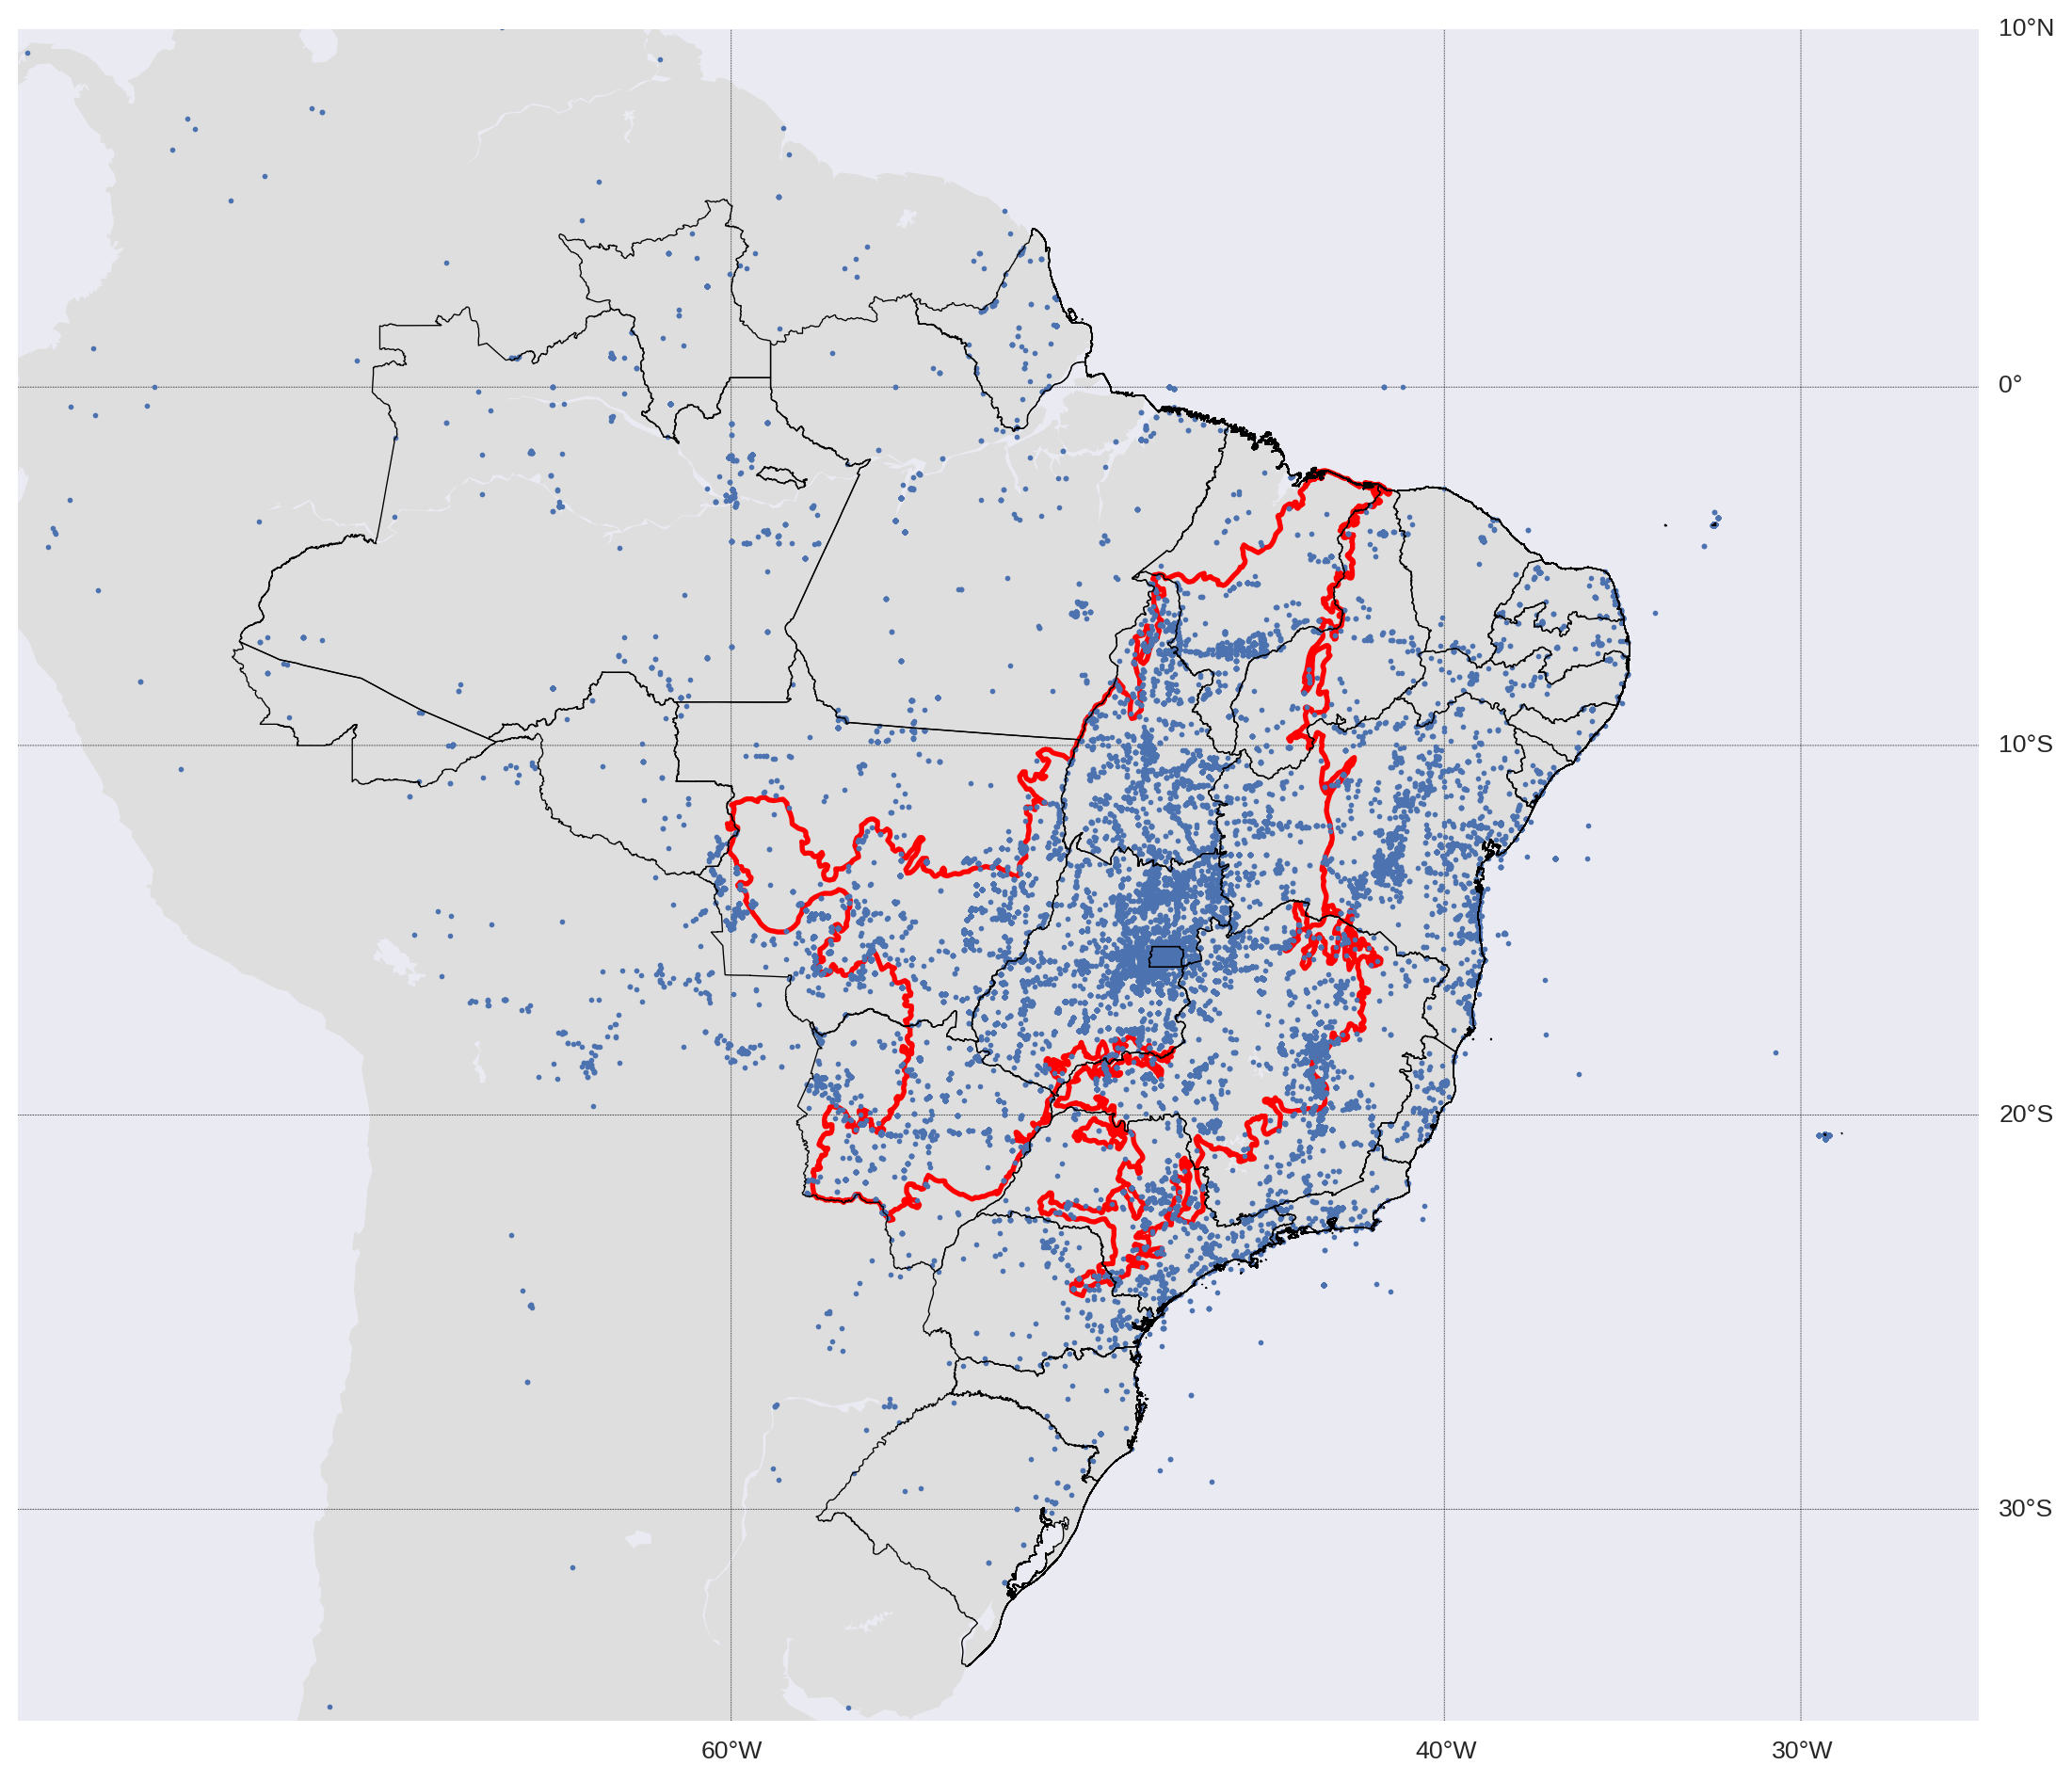
\includegraphics[width=\linewidth]{figures/occurrence_map.png}
\caption[Geographic distribution of the occurrences from the UB Herbarium dataset near the Brazilian territory.]{Geographic distribution of the occurrences from the UB Herbarium dataset near the Brazilian territory. Records without geospatial issues are placed in the map as blue dots. The area outlined in red represents the boundaries of the Cerrado biome.}
\label{fig:occurrence_map}
\end{figure}

Most records deposited in the UB herbarium were collected in Brazil ($94.47\%$), from which the Federal District (DF) is the most sampled federative unit despite its relatively small area~(Figure \ref{fig:recsbycntrystate}(b)).
Records in the Federal District comprise $30.56\%$ of those falling within the Brazilian territory. 
Other states with relatively high collecting effort are Goiás ($22.10\%$), Minas Gerais ($14.51\%$), and Mato Grosso ($7.86\%$), which, together with the Federal District, correspond to $75\%$ of all records from Brazil in the UB herbarium.
Such a geographical bias in the occurrence distribution can be explained by the fact that UB is physically located at the University of Brasilia, making it more viable for associated collectors to perform collecting expeditions in nearby locations.
Moreover, as UB is a national reference herbarium for species occurring the Cerrado biome, botanists working in Cerrado areas nearby might become more inclined towards depositing their recordings in that institution.
Figure~\ref{fig:occurrence_map} shows that UB records are more densely concentrated within the Cerrado biome, mostly in the Central Brazil region.
The UB herbarium also includes a total of $10,252$ records from other countries~(Figure \ref{fig:recsbycntrystate}(a)), which are derived from exchanges with foreign herbaria (under the curatorship of \textit{Dr. George Eiten}~\cite{florescer}) and from international recording expeditions performed by collectors associated with the UB herbarium.

\begin{figure}[!htb]
\centering
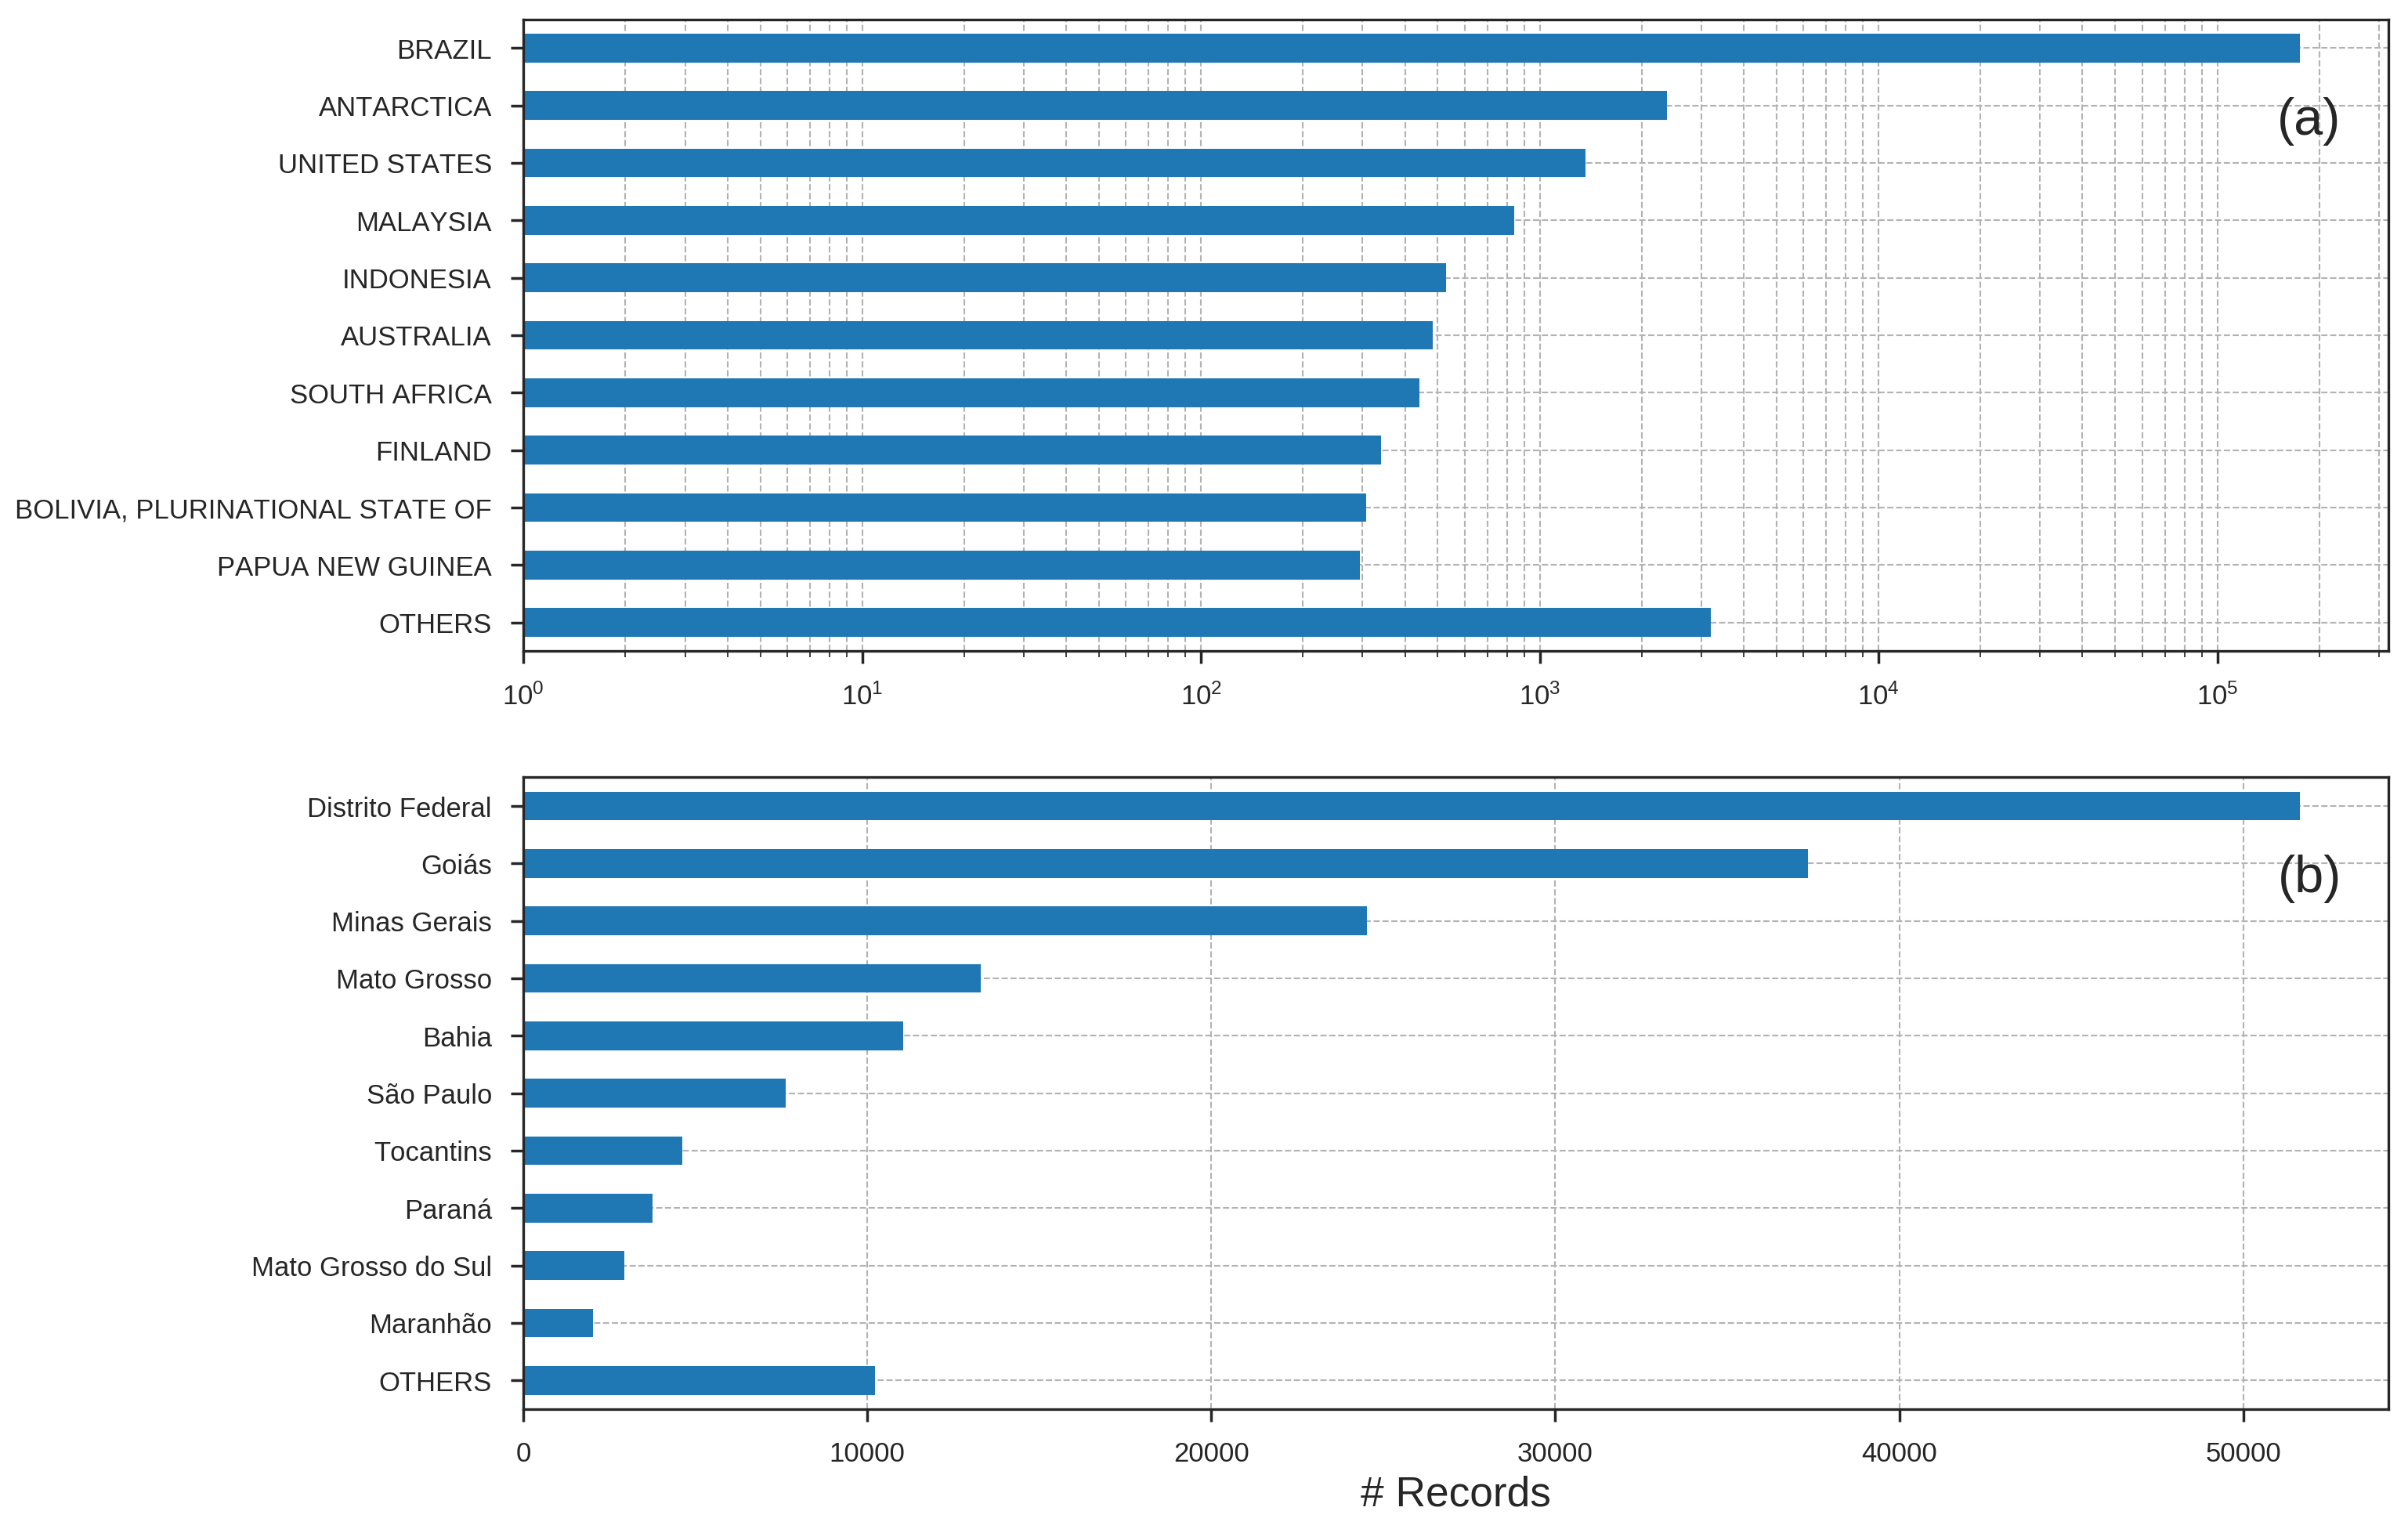
\includegraphics[width=\linewidth]{figures/recs_by_cntry_state.png}
\caption[Top-10 countries and Brazilian states with most occurrence records deposited in the UB herbarium]{Top-10 countries (a) and top-10 Brazilian states (b) with most occurrence records deposited in the UB herbarium. Records from countries and states beyond the $10th$ position in the respective ranks are summed and assigned to \textit{OTHERS}.}
\label{fig:recsbycntrystate}
\end{figure}

\art{Parei revisao aqui}  

% --------------------------
% Temporal characterization
\paragraph*{Temporal distribution.}

Although preprocessing routines in GBIF also include the interpretation of date-time values in the \textit{eventDate} field, no flags regarding date-time inconsistencies have been assigned to any of the records from the UB dataset.
A total of $181254$ records, comprising $97.86\%$ of the $185301$ records we explored, contain information about their collection dates.
The temporal distribution of the records spans the period from year $1800$ up to $2017$, although a more intensive collection activity starts around year $1960$ (Figure \ref{fig:ub_records_timeseries}).
In fact, the vast majority of records ($96.11\%$) are concentrated within the period from $1960$ to $2017$ (an average of $3000$ records per year), whereas the period from $1800$ to $1959$ includes only $3.9\%$ of the records, with an average of $45$ records per year.
Moreover, the number of records accumulated during the last $30$ years (from $1988$ to $2017$) is approximately equal to the number of records from $1800$ to $1987$ ($188$ years). 
Three peaks of activity are most pronounced in Figure \ref{fig:ub_records_timeseries}.
The first is around years $1966$ and $1968$, the second around $1988$, and the third around $2012$.

\begin{figure}[h!]
\centering
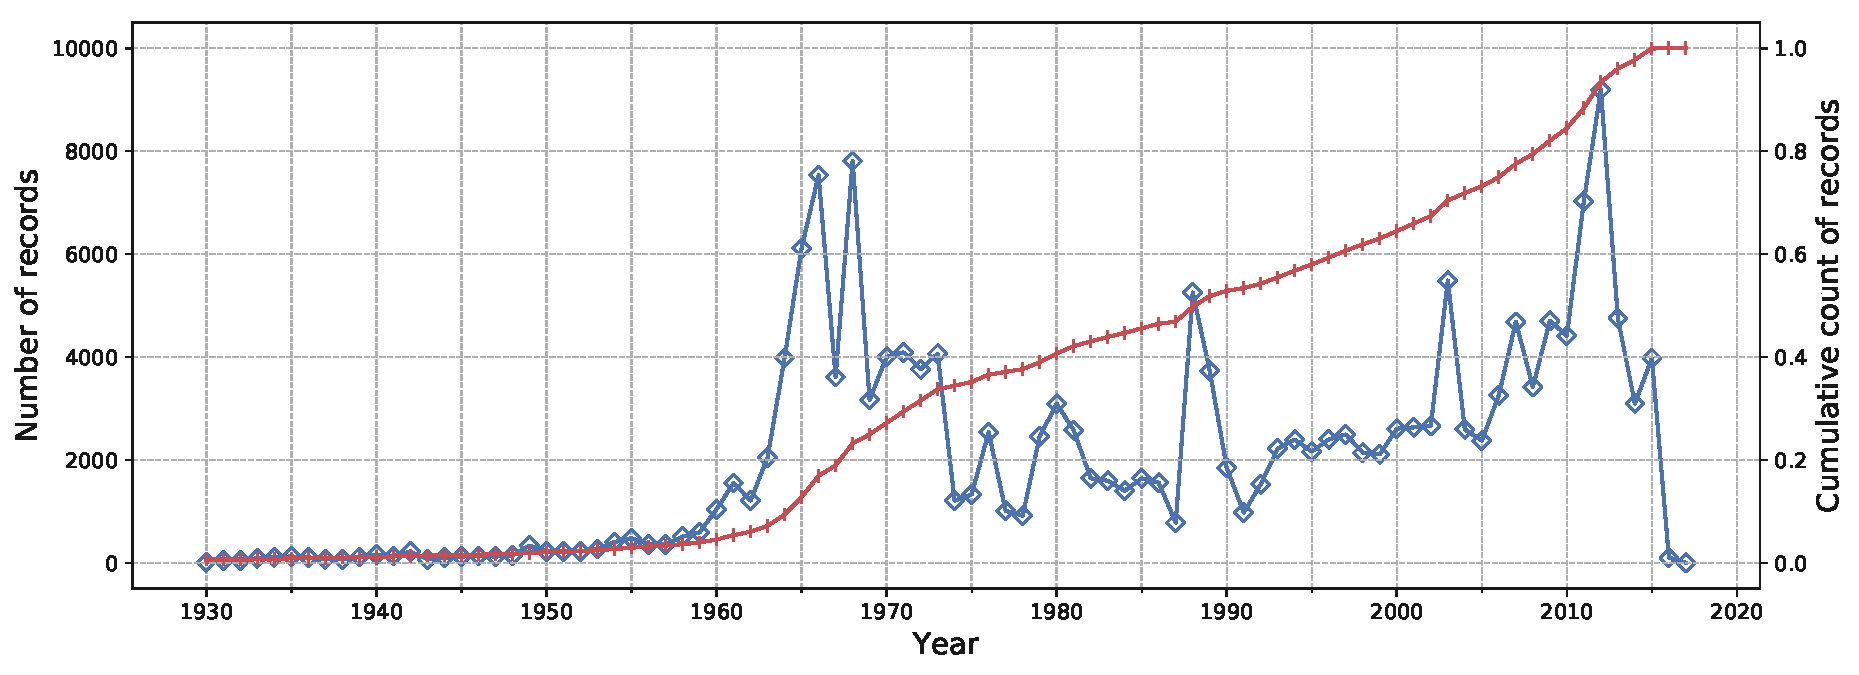
\includegraphics[width=\linewidth]{figures/casestudy_ub/ub_records_timeseries.pdf}
\caption[Recording activities registered in the UB herbarium aggregated by year, since $1930$.]{Recording activities registered in the UB herbarium aggregated by year, since $1930$. Both the absolute (blue line) and the cumulative (red line) record counts for each year are shown.}
\label{fig:ub_records_timeseries}
\end{figure}


%\clearpage


% ---------------------------
% ---------------------------
% Network models construction
\section{Network models construction}

In this section we describe the main features of the Species-Collector Network (SCN) and the Collector CoWorking Network (CWN) constructed from the UB herbarium occurrences dataset.
Using these models we explore the diversity of recording behaviors of the collectors who contribute to UB, in terms of their taxonomic preferences and collaborativeness during collecting expeditions.
We start by describing our data preparation routine, necessary for improving the quality of the network models.

\subsection{Data preparation} \label{section:ub_data_preparation}
Before we could use the UB occurrences dataset for actually building the network models, we submitted the tabular dataset to some data filtering and transformation routines.
The data preparation process consisted of 
(\textit{i}) selecting occurrence records from which relevant social ties could be derived for both network models; 
(\textit{ii}) extracting atomized collectors names from the \textit{recordedBy} field, which originally contains a string of names;
(\textit{iii}) normalizing the extracted collectors names to obtain their id's;
(\textit{iv}) resolving collectors names inconsistencies and mapping names variants to entities;
(\textit{v}) filtering out inadequate collectors names. %such as et al, incognito... performed after the network is built

In the first step we initially removed all records with missing values for either fields \textit{recordedBy} or \textit{scientificName}, as these are both critical for the construction of the network models.
In order to build the SCN at the taxonomic resolution of \textit{species} we selected records for which the taxonomic identity could be resolved at that level, \textit{i.e.}, at the resolutions of \textit{form}, \textit{variety}, \textit{subspecies} and \textit{species}. 
This subset of records corresponds to approximately $82\%$ of the original dataset (a total of $152379$ records, as shown in Table \ref{table:dset_taxonomicres_counts}).
All records with taxonomic resolution higher than \textit{species} (from \textit{genus} to \textit{kingdom}) were not used for the construction of the networks.
Although the taxonomic resolution of records is not relevant at all for the construction of the CWN model (edges are built exclusively using cliques of collectors, a process described in section \ref{section:cwn_construction_fromdata}), we chose to use the same set of records we used for building both models.

The names atomization step consists of iterating each record from the UB dataset and splitting the corresponding string containing collectors names, originally stored in the \textit{recordedBy} field. 
The process originates a list of strings for each record, containing atomic names for each collector associated to it.
A new field named \textit{recordedBy\_atomized} is created for holding the lists of atomic names, and is later used to construct the network models.
We splitted the strings on the semicolon character (` ; '), as it is used as the delimiter for the majority of entries.
In some few occurrences, however, names are delimited by other characters, for instance ` , ', ` / ' and ` \& '.
We dealt with these cases by replacing inconsistent delimiters manually and storing the changes in a separated file, without modifying the original dataset.


In order to obtain unicode identities for collectors, we defined a unicode normalization function, which is executed on collectors names strings upon network construction (step \textit{iii}).
Each name is initially split in its two component parts (see \ref{section:ub_exploration}), using the comma character as the delimiter.
Next, each part of the name is passed into the normalization function, which forces all characters to lowercase and removes any accents, periods and spaces. 
Finally the name is recomposed by joining the first initials to the last name with a comma.
For instance, name `\textit{Simão, J. S.}' would be normalized to `\textit{simao,js}'.
Names were mapped to their respective normalized forms and were stored in a \textit{names map} file, which was later passed in to the constructor methods that built the network models.
A table mapping the identities of some of the main collectors from UB to their respective names is presented in Appendix \ref{appendix:collectors_ids}.
However, we still faced the problem of resolving names inconsistencies (step \textit{iv}).
If a collector is associated to multiple names variants, she gets consequently represented as multiple entities in the network, which should be avoided as to ensure the semantic correctedness of the models.
For dealing with these issues, we included new entries in the same \textit{names map}, keying variants of each name are to their ``correct forms''.
Finally, after the networks were built, the last step was to remove entities which we considered to be ``noise'' in the network, such as `\textit{etal}' (from \textit{et. al}), `\textit{incognito}', `\textit{ignorado}', `\textit{ilegivel}' or `\textit{?}'.






% ==========================
% Species-collectors Network
% --------------------------
\subsection{The UB Species-Collector Network} \label{section:ub_scn}

The SCN model of the UB herbarium had a total of $6768$ collectors and $15344$ species nodes, with a total of $142647$ undirected edges connecting nodes from opposite sets. 
Average degree for the collectors and species set are respectively $21.08$ and $9.30$.

\paragraph{Connected components.}
The network is composed of a total $351$ connected components, the largest of which (the giant component, or $c_1$) contains the majority of nodes in the network ($93.6\%$ of the collectors and $95.0\%$ of the species). 
From a collector's perspective, the requirement for it to belong to the giant component is that it must have collected at least one species in common with another collector who is already included in the giant component. The same reasoning applies to species nodes, by observing the inverse relationship.
Apart from the giant component, most other connected components contain as few as two or three nodes, representing collectors who have never recorded a species in common with any collector from $c_1$; and conversely, species that have never been collected by any of those $c_1$ collectors.
One of those $350$ remaining connected components, however, is considerably larger than the others, with a total of $3$ collectors and $141$ species. We refer to it as the second largest component ($c_2$) throughout this section.

Among all the records that form the giant component, $95.2\%$ are from Brazil, from which $53\%$ were recorded either in the Federal District or in the state of Goiás. 
Also, $c_1$ is mostly composed of species from phylum \textit{Tracheophyta} ($88\%$ of all records), followed by phylum \textit{Bryophyta} (mosses), comprising $8\%$ of the records. 
Component $c_2$, on the other hand, is represented by algae (phyla \textit{Charophyta}, \textit{Chlorophyta}, comprising $91.6\%$ of all records), bacteria (phylum \textit{Cyanobacteria} ($4.3\%$)) and other microscopic eukariotic organisms (phyla \textit{Euglenozoa}, \textit{Myzozoa} ($4.1\%$)), which are taxonomically distinct from the vast majority of species in the herbarium.
In addition, all records composing $c_2$ were collected in the Federal District.
The remaining components ($c_3,c_4,..., c_{351}$) include a total of $431$ distinct collectors and $446$ distinct species, resulting from records from many other countries than Brazil ($79\%$ of the records).
The most representative country is the United States, with $23.9\%$ of the records, followed by Brazil (with $21\%$). 
Considering the records from within Brazil, only $7.8\%$ of them were collected in the Federal District. Most of them ($59.2\%$) are from the southeast region, among which the state of São Paulo is most representative ($52.5\%$).

We have hypothesized some possible explanations for the existence of so many small connected components in the UB herbarium SCN with such characteristics. First, they could be a consequence of specimen exchange, a practice that is widely adopted among herbaria for collaboratively diversifying and distributing their collections \cite{Groom2014}. Exchange materials are typically duplicated exsiccates collected in field that a sender institution dispatches to a receiver institution. The receiver institution then incorporates those materials to its scientific collection, and ocasionally sends back to the other institution some duplicate exsiccates of its own.
From the receiver herbarium viewpoint the inclusion of records from exchanges usually adds new species and collectors, for they are a sample reflecting the sender institution's purpose and the interests of people associated to it. If both the collectors and species from such records were previously inexistent in the receiver collection, no links to $c_1$ or to any other connected component that already exists are formed. These records thus get included into its SCN network as nodes and edges composing new small connected components. We should overstate, however, that including exchange records does not necessarily create new connected components. New species or collectors could be included in $c_1$ in case either the species or at least one of the collectors associated to the exchange record are already linked to it.

A second situation that could potentially lead to isolated components in the network is when there are groups of very specialized collectors sampling very specific and distinct groups of organisms. 
Cryptic organisms such as algae, fungi and mosses are examples of groups which tend to be overlooked by botanists who are not directly interested on them. 
If collectors who record such groups also show a very high specificity towards them, it gets more likely that they lack links to other species which are more commonly recorded by the rest of the collectors, thus forming structures that are weakly linked (if not detached) to the giant component. 
In case these collectors regularly deposit their materials in the herbarium it would be natural to observe them composing connected components with a relatively large number of species.
The connected component $c_2$, for instance, includes \textit{Ana Lúcia Tostes Leite} (\textit{leite,alta}), one of the herbarium's most relevant continental algae collector as shown in Table \ref{table:ub_collectors_florescer}.
She holds a total of $2757$ records, from $87$ distinct species, all of them being charophytes, a division of green algae (Figure \ref{fig:ub_scn_agg_family_general}, within polygon $ii$).



\paragraph{Number of species per collector.}
Collectors contributing to the UB herbarium have, in average, recorded and successfully deposited approximately $21.1$ distinct species in that collection during their careers (Table \ref{table:ub_scn_degrees}). This value is obtained by computing the average degree $\langle k_{col} \rangle$ from all nodes in $S_{col}$ set, and would be equivalent to the expected number of species for a randomly selected collector if the SCN were a random network \cite{Albert2002}.
However, by visually inspecting the degree distribution of collectors in Figure \ref{fig:ub_scn_degree_dist}(b and d) we realize that the vast majority of collectors have recorded very few species. In fact, around $86.7\%$ of the collectors have degrees below or equal $floor(\langle k_{col} \rangle)$, and around $79\%$ have recorded $10$ or fewer species.
On the other hand, there are also some few collectors who have recorded much more species than the average, as it is the case of \textit{Howard S. Irwin} (\textit{irwin,hs}), with a total of $4535$ records of distinct species; and \textit{Carolyn E. B. Proença} (\textit{proenca,ceb}), with $1888$ distinct species. Such nodes holding a very high number of connections in the network are called hubs.

\begin{table}[t]
\caption[Degree centrality metrics for the UB SCN model.]{ Degree centrality metrics for the UB SCN model. For each nodes set the total number of nodes, average degree $\langle k \rangle$, top-10 highest-degree nodes and their respective degree $k$, weighted degree $k_w$ and normalized degree $k^*$ are listed.}
\begin{center}
	\caption{Some degree metrics for the UB SCN model. For each nodes set the total number of nodes, average degree $\langle k \rangle$, top-10 highest-degree nodes and their respective degrees $k$ are listed. We define $k^*$ as the maximum possible degree of a nodes set, a metric that represents the degree of a hypothetical node which is connected to every single node from the complementary set. Therefore $k/k^*$ is the proportion of nodes from the complementary set a given node is linked to.}
  \begin{center}
  \begin{tabular}{l c c c c c}
    & num of nodes & $\langle k \rangle$ & top-10 & $k$ & $k/k^*$ \\
   \hline    collectors & 6768 & 21.08 &
   \begin{tabular}[t]{{@{}c@{}@{}}}irwin,hs\\heringer,ep\\anderson,wr\\proenca,ceb\\ratter,ja\\faria,jeq\\eiten,g\\souza,rr\\harley,rm\\santos,rrb\end{tabular} &
   \begin{tabular}[t]{{@{}c@{}@{}}}4535\\2586\\2156\\1888\\1803\\1681\\1586\\1549\\1514\\1502\end{tabular} &
   \begin{tabular}[t]{{@{}c@{}@{}}}0.30\\0.17\\0.14\\0.12\\0.12\\0.11\\0.10\\0.10\\0.10\\0.10\end{tabular} \\ \\
    species & 15344 & 9.30 &
   \begin{tabular}[t]{{@{}c@{}@{}}}\textit{Myrcia splendens}\\\textit{Myrcia guianensis}\\\textit{Eugenia punicifolia}\\\textit{Casearia sylvestris}\\\textit{Palicourea rigida}\\\textit{Myrcia tomentosa}\\\textit{Qualea parviflora}\\\textit{Solanum lycocarpum}\\\textit{Piper aduncum}\\\textit{Miconia albicans}\end{tabular} &
   \begin{tabular}[t]{{@{}c@{}@{}}}388\\335\\266\\258\\241\\239\\232\\228\\209\\201\end{tabular} &
   \begin{tabular}[t]{{@{}c@{}@{}}}0.06\\0.05\\0.04\\0.04\\0.04\\0.04\\0.03\\0.03\\0.03\\0.03\end{tabular} \\ 
  \hline
  \end{tabular}
  \end{center}
  \label{table:ub_scn_degrees}

\end{center}
\label{table:ub_scn_degrees}
\end{table}

  \begin{figure}[t]
  	\centering
    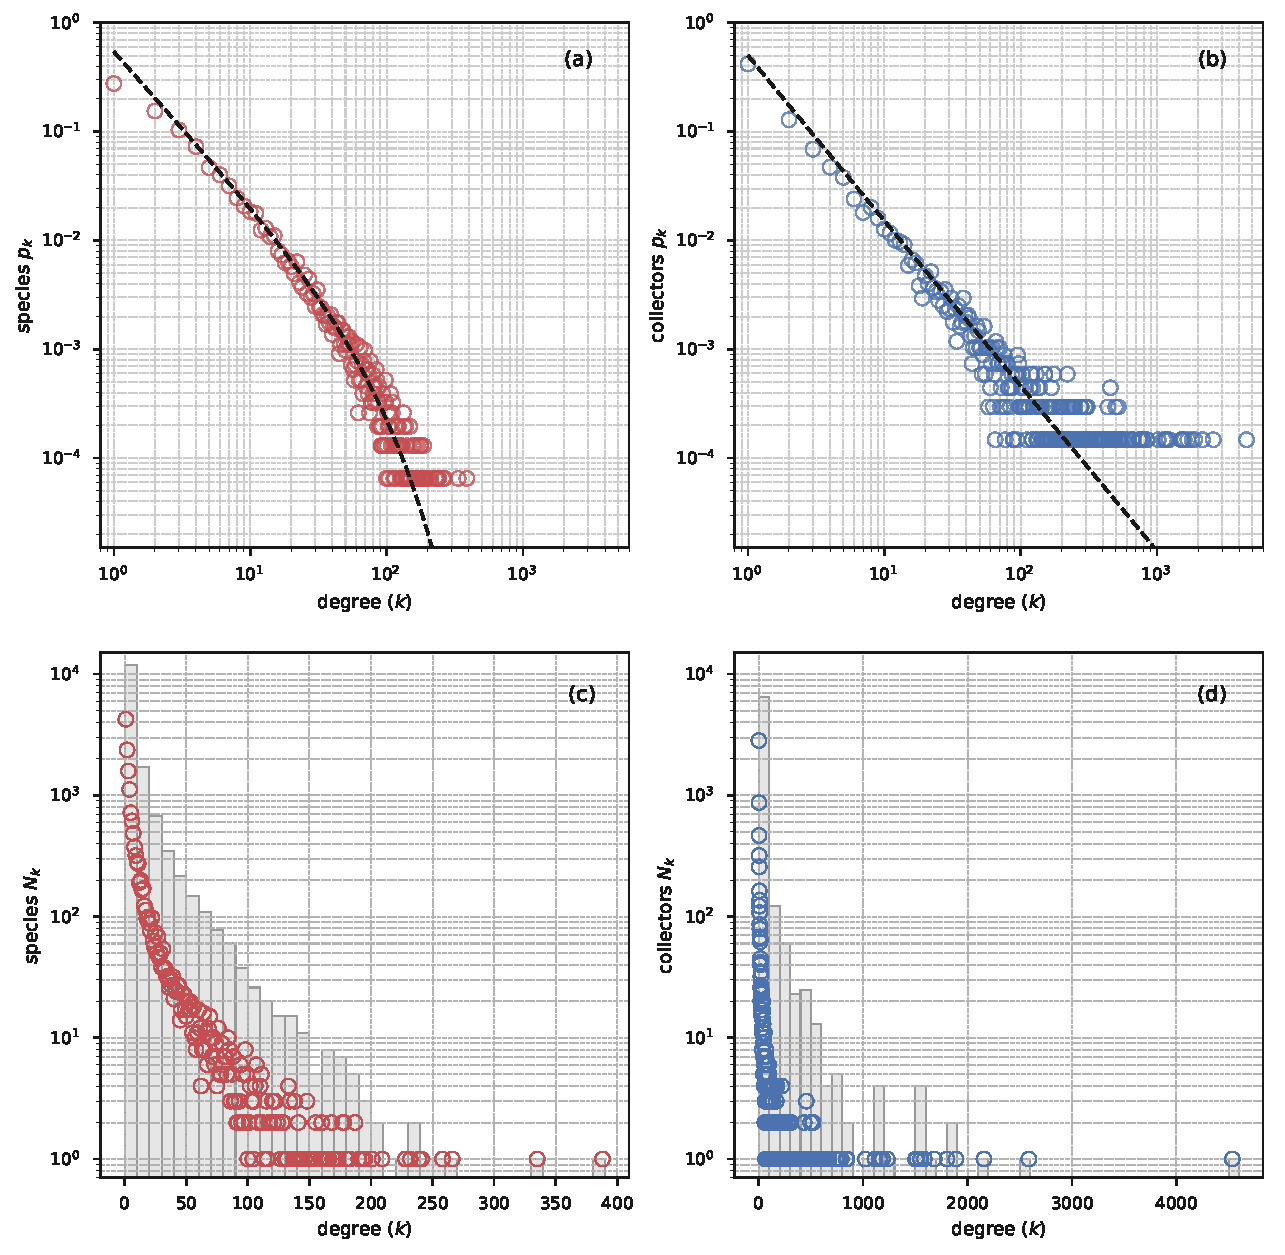
\includegraphics[width=\linewidth]{figures/casestudy_ub/scn_degree_dist}
    \caption[Degree distribution for both species and collectors nodes.]{Degree distribution for both species ($a$ and $c$) and collectors ($b$ and $d$) nodes. The upper row plots show the probability $p_k$ of finding nodes with each degree value, using a log-log scale. The dashed curves represent power laws ($a$ has a tail cutoff) that best fit the SCN data, with $\alpha=1.38$ and $\alpha=1.52$ for plots $a$ and $b$, respectively. The exponential cutoff in $a$ is obtained by using $\lambda=0.014$. Plots in the lower row show the total number $N_k$ of nodes with each degree value, using a lin-log scale for enhancing interpretability. Histograms in the background group collectors using bin sizes $s=10$ and $s=100$ for plots $c$ and $d$, respectively.}
    \label{fig:ub_scn_degree_dist}
  \end{figure}

As opposed to random networks, in which extremely well connected nodes are unlikely to coexist with a large number of extremely poorly connected ones, the degree distribution observed for collectors in the UB SCN is better approximated by a power law $p(k) \sim k^{-\alpha}$, typically observed in many large real-world networks with the scale-free property \cite{Barabasi1999a}. 
The dashed line in figure \ref{fig:ub_scn_degree_dist}b is a power law fit for the degree distribution of nodes from $S_{col}$, with $\alpha=1.52$. 
An apparently similar heavy-tailed distribution was recently reported by \citeonline{Daru2017} while investigating sampling bias in the digitized datasets of three distinct herbaria from Australia, South Africa and the United States.
  
Other useful degree centrality metrics shown in Table \ref{table:ub_scn_degrees} are the weighted degree $k_w$ and normalized degree $k^*$. The weighted degree for each collector node is computed by summing up weights assigned to each of the node's edges. Edges can be weighted according to any chosen attribute of its own, depending on the aspect of the connection the user wants to emphasize. Here we use the \textit{count} attribute, which holds the number of times the association between a collector and a species occurs. Formally, $k_w^{(u)} = \sum_{v} count(e_{u,v})$ for $v \in$ $neighbors(u)$. Differently from the degree, which gives the number of distinct species that have been recorded by a collector, the weighted degree of a collector can be interpreted as the total number of specimens (or occurrence records) collected by him/her. It is also worth noting that the value of $k_w$ of a node is equivalent to its \textit{count} attribute (not to be confused to the homonymous attribute of edges).

The intuition behind the normalized degree $k^*$ of a collector is the fraction of species from the entire $S_{sp}$ set it is connected to. We compare the degree of the node to the maximum degree value that would be possible for nodes in the same set. In a bipartite model it turns out to be the node's degree divided by the size of the opposite set. Therefore, $k^{*(i)} = \frac{k^{(i)}}{|S_{sp}|}$, for a node $i \in S_{col}$. 
As stated by \citeonline{Borgatti2015}, the advantage of using this normalized metric over the non-normalized degree $k$ is that it allows us to numerically compare centrality scores across nodes sets independently of their respective sizes. 
In our case collectors hubs tend to be more central than species hubs. The top collector \textit{irwin,hs} is linked to $30\%$ of the total diversity of the herbarium species, whilst the top species \textit{Myrcia splendens} has been recorded by $6\%$ of the herbarium collectors (Table \ref{table:ub_scn_degrees}). 



\paragraph{Number of collectors per species.}
For the species nodes set ($S_{sp}$), the average degree $\langle k_{sp}\rangle \approx 9.5$, which can be interpreted as that species in the UB herbarium have been collected by approximately $9.5$ distinct collectors, in average. 
The total number of times each species has been recorded and the percentage of collectors that have recorded them at least once are given by the $k_w$ and $k^*$ metrics, respectively (Table \ref{table:ub_scn_degrees}).

The degree distribution for species nodes (Figure \ref{fig:ub_scn_degree_dist}(a and c)) is similar to the distribution for collectors nodes, with a majority of very low degree nodes coexisting with a few hubs.
Most species (around $76.7\%$) hold degree values below or equal $floor(\langle k_{sp}\rangle)$, meaning they've been recorded by $9$ distinct collectors or less.
Yet, there are also some species that have been recorded by many more collectors than the average, as it is the case of \textit{Myrcia splendens} and \textit{Eugenia punicifolia}. Those top-10 species (Table \ref{table:ub_scn_degrees}) are in fact reasonably well-known, common and easily detectable. Typical from cerrado physiognomies, \textit{Solanum lycocarpum} (\textit{lobeira}), \textit{Palicourea rigida} (\textit{chapéu-de-couro}), \textit{Qualea parviflora} (\textit{pau-terra}) are examples of species that are both very conspicuous and easy to identify.

A particularity that can be observed in the species degree distribution is the existence of a sharp tail decrease in the probability curve towards the highest degree nodes (Figure \ref{fig:ub_scn_degree_dist}a), known as a tail cutoff.
This behavior can be better adjusted by using a slight variant of the power law function $p(k) \sim e^{-\lambda k} k^{-\alpha}$, which is obtained by simply including an exponential term in the function. We call this variant a truncated power law function, as the degree distribution of nodes is not scale-independent.
Truncated power-laws have been also reported by \citeonline{Newman2004} for scientific collaborations networks. 
As there is an evident limitation on the number of papers scientists are able to publish during an interval, Newman has attributed this behavior to the limited time window used in his studies. 
However, the same behavior has also been observed in other real world networks, in which the formation of a very high number of links on any node is constrained by some physical factor, specific to each system \cite{Albert2002}. 
In the case of SCNs, the exponential cutoff might be due to the fact that as the representativity of species in the herbarium increases, collectors become less inclined towards collecting those species in the future. 
The dashed curve in Figure \ref{fig:ub_scn_degree_dist}a represents a truncated power with parameters $\alpha=1.38$ and $\lambda =0.014$, which was fit to the species degree distribution data.


\paragraph{How densely connected are species and collectors?}
The density of the network is the ratio between the number of actual number of edges in the network and the maximum possible number of edges, in case every collector were linked to every species. This metric informs us how far the network is of being complete, in which case its density becomes $d=1$. For a bipartite network, density can be computed as $d = \frac{|E|}{|S_{col}| |S_{sp}|}$, where $|E|$ is the number of edges in the network and $|S_{col}|$ and $|S_{sp}|$ are the number of collectors and species, respectively.
%
The observed density for the overall UB species-collectors network is approximately $1.37 \times 10^{-3}$, meaning that the probability that we find an edge linking two arbitrary nodes from opposite sets is about $0.14\%$. Additionally, as shown in Figure \ref{fig:ub_scn_tax_agg_curves}, network density increases as we perform taxonomic aggregations onto successively higher-hierarchy ranks.
%
In most social networks, however, not all regions are equally dense, as entities usually do not connect to others randomly. Instead, entities with similar attributes or interests are more likely to establish new ties with each other than with dissimilar ones, leading to the formation of communities in the network.
% find parameters for network density (compare with other networks in literature)


\paragraph{Communities of common interests.}
Communities in SCNs are formed by groups of collectors who are more interested towards particular subsets of species than are other collectors, external to the group.
As the number of edges linking members of a community with other members tends to be greater than those connecting members to non-members, communities can be visually detected as distinguished clusters of nodes in the network when using force-directed algorithms \cite{Jacomy2014} for graph layout.

As the size of the UB SCN is relatively big for it to be informative in a static figure, we summarized the network in two steps.
First we aggregated the SCN onto the \textit{family} rank following the routine described in section \ref{section:taxonomic_aggregation}, as it would be impractical to draw relevant conclusions from the network if every single species were plotted in the figure.
By performing the taxonomic aggregation, we reduced the number of $S_{sp}$ nodes (taxa) from $15344$ to $474$, although the number of edges (from $142647$ to $43803$) did not decrease in the same proportion (Figure \ref{fig:ub_scn_tax_agg_curves}).
This incurred in a $10 \times$ increase in network density, from $1.37\times 10^{-3}$ to $1.36\times 10^{-2}$.
In the second step of the summarization routine we removed collectors-families ties which occurred less than $20$ times throughout the entire dataset by filtering edges based on their \textit{count} attribute.
As this edges filtering routine resulted in many isolated collectors, most of which novice collectors with low absolute recording counts, we also omitted them as to improve figure readability.

\begin{figure}[!ht]
  	\centering
    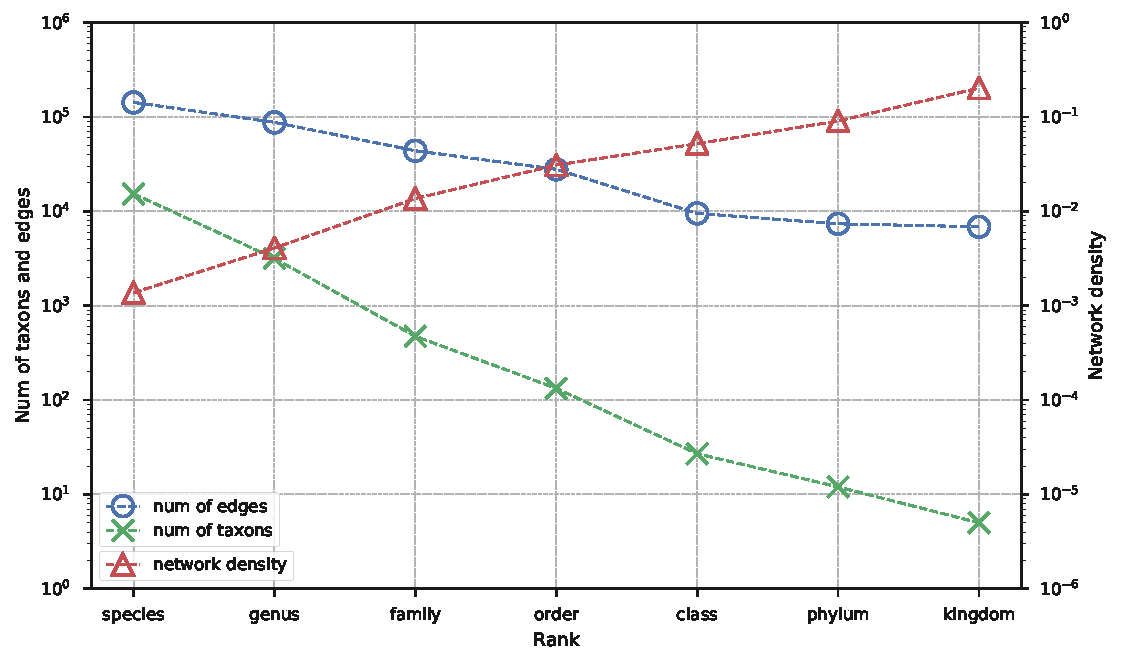
\includegraphics[width=\linewidth]{figures/casestudy_ub/scn_tax_agg_curves.pdf}
    \caption{ Number of taxa ($S_{sp}$ nodes), edges and network density for the UB SCN aggregations onto successive taxonomic ranks. }
    \label{fig:ub_scn_tax_agg_curves}
  \end{figure}

\afterpage{
  \begin{figure}[!ht]
  	\centering
    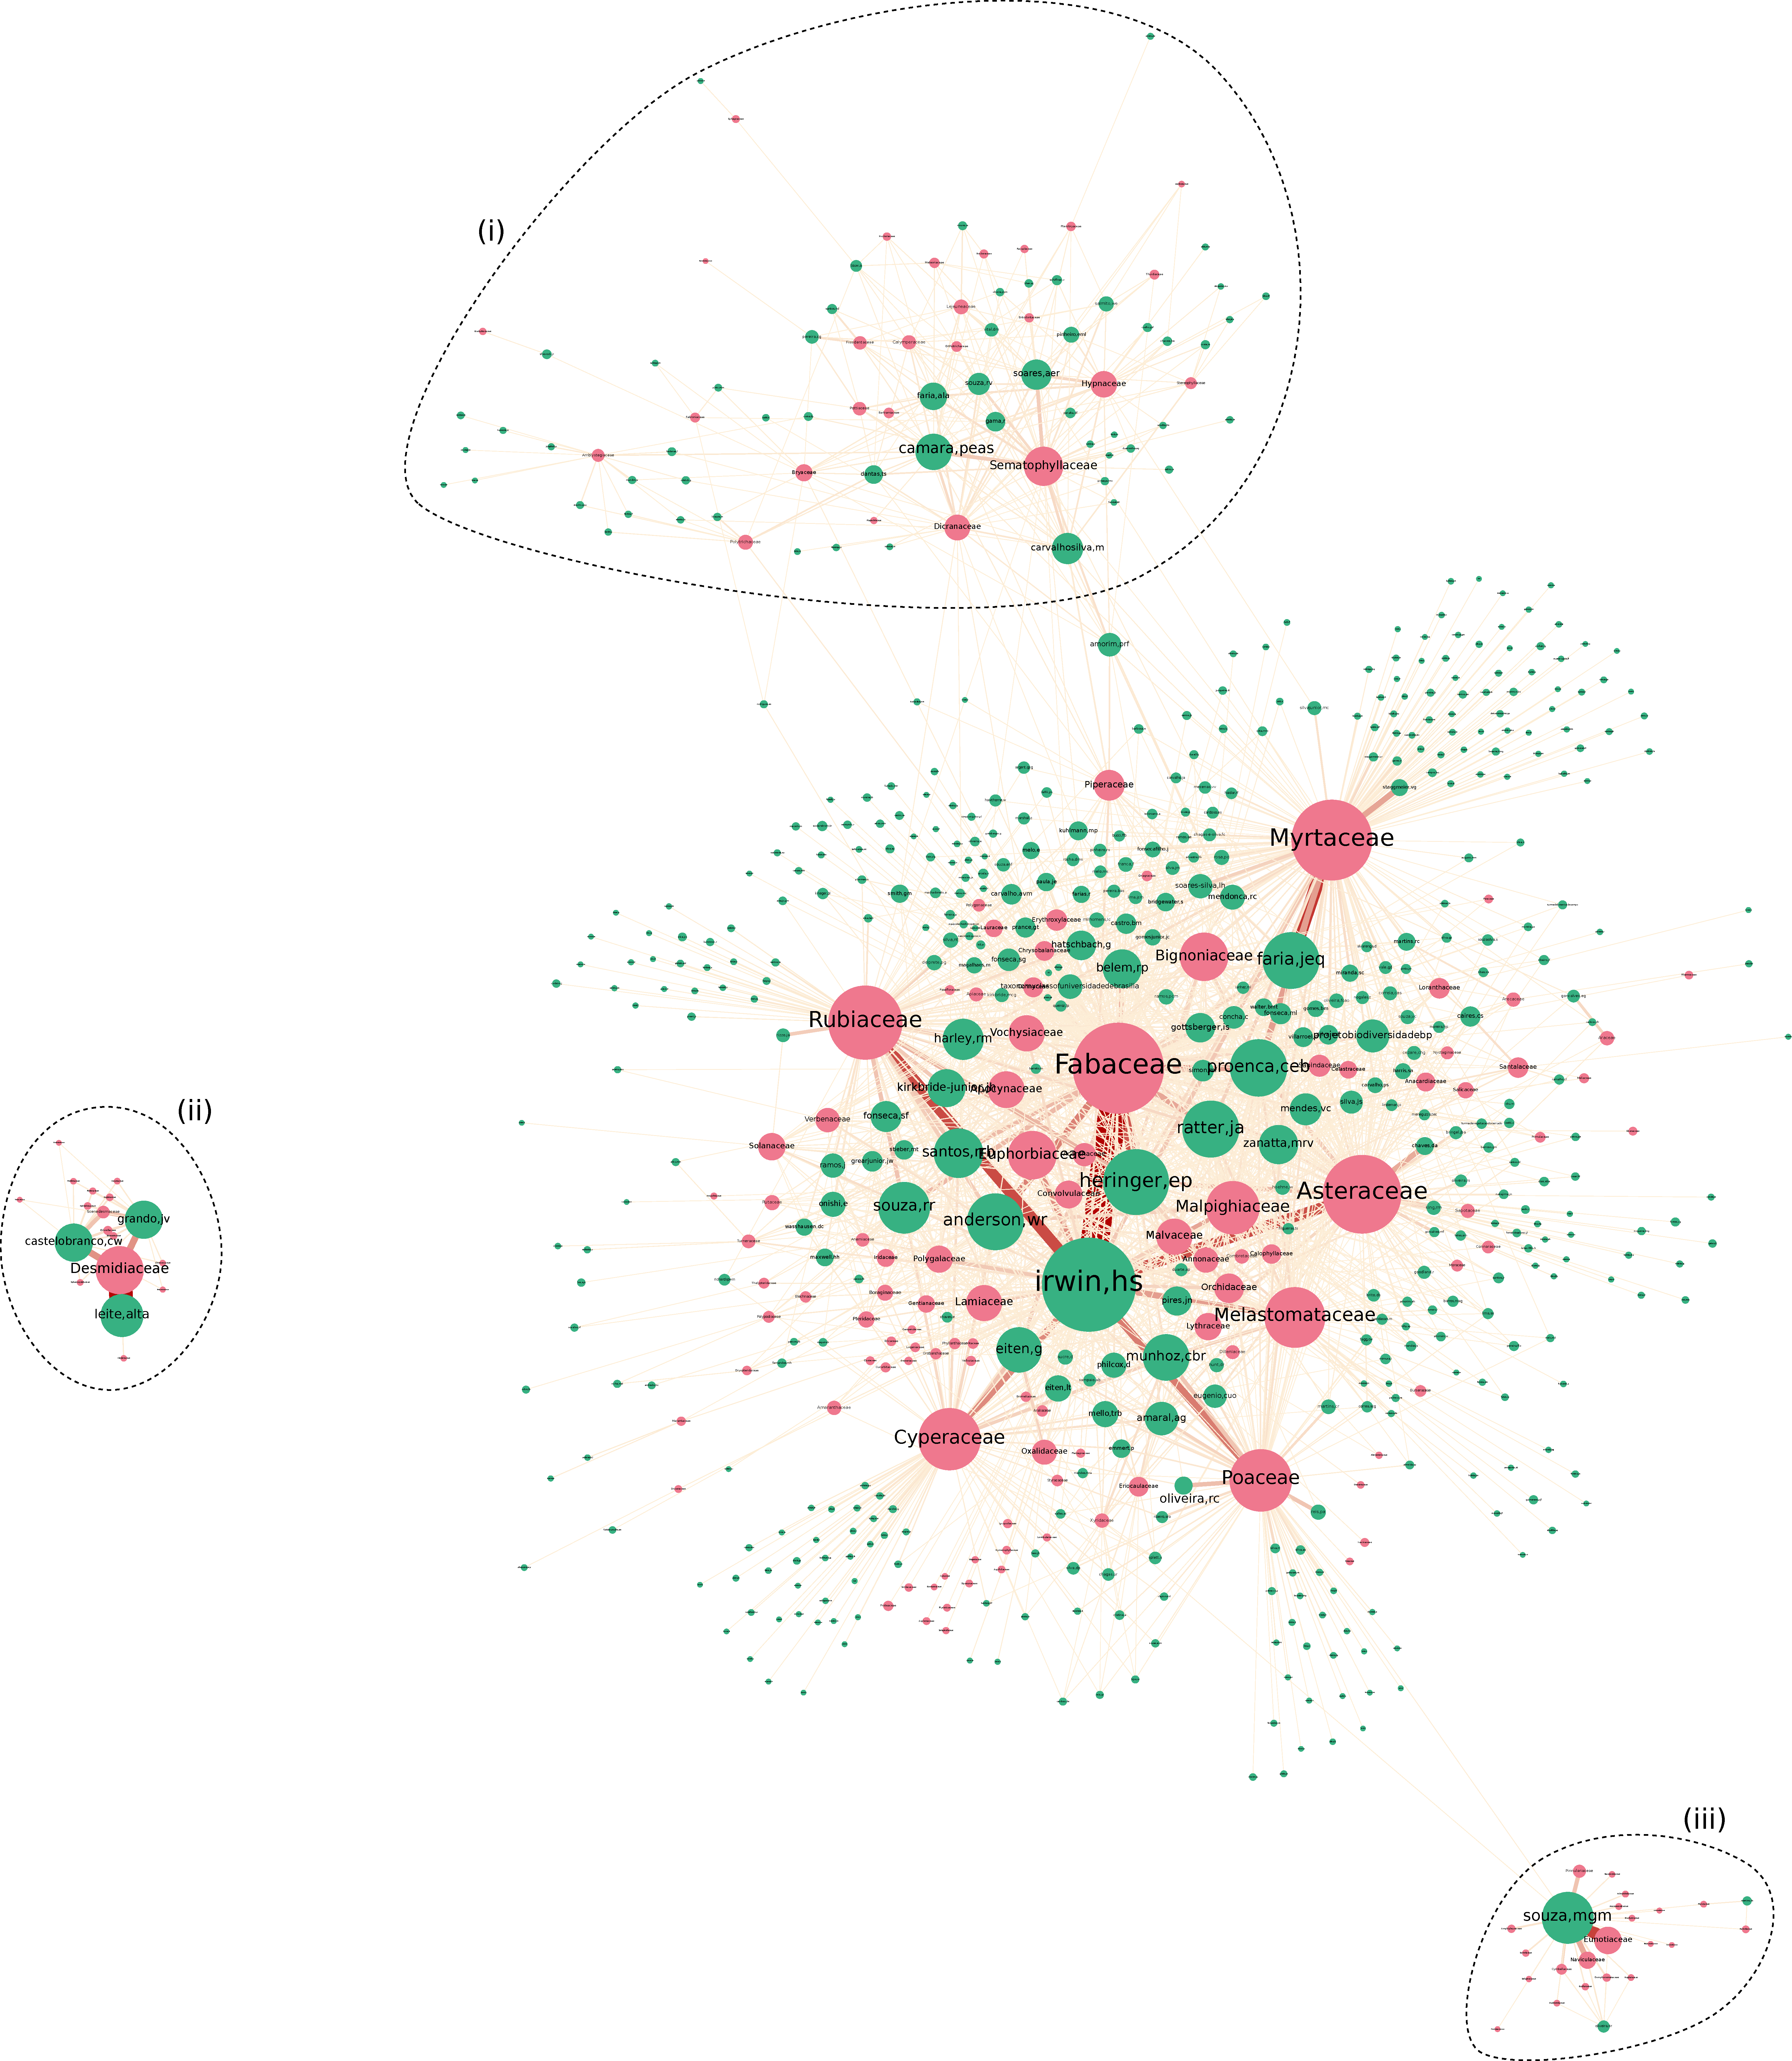
\includegraphics[width=\linewidth]{figures/casestudy_ub/scn_agg_family_general.pdf}
    \caption[General aspect of the UB SCN taxonomically aggregated at the family rank.]{ General aspect of the UB SCN taxonomically aggregated at the family rank. Species and collectors are respectively represented as pink and green nodes, and edges are weighted according to their \textit{count} attribute. Nodes sizing is based on their \textit{count} attribute, whilst edges color and width reflect their weight. For improving visualization we first filtered out edges with weight lower than $20$ and then omitted isolated nodes from the resulting graph. Nodes within poligons $(i)$, $(ii)$ and $(iii)$ compose visually distinguishable communities. Graph layout was computed using the \textit{ForceAtlas2} algorithm \cite{Jacomy2014}. For a better visualization experience refer to the interactive graph in the author's personal web page\footnotemark. }
    \label{fig:ub_scn_agg_family_general}
  \end{figure}
  \footnotetext{ \url{https://pedrosiracusa.github.io/networks/ub_scn_agg_family} }
}

Three communities are visually distinguishable from the central region of the network, which we'll refer to as the network core (Figure \ref{fig:ub_scn_agg_family_general}).
Although the network core could be considered a community \textit{per se}, we prefer to think of it as a region that best reflects the overall interests of the majority of the collectors contributing to the herbarium.
Nevertheless, collectors from the network core still vary considerably regarding their recording interests, as it can be verified by inspecting the sets of taxa they're linked to and the strength of their connections. 
Those who have sampled organisms from many distinct families (and are thus considered to display a more generalist collecting behavior) are placed more centrally in the network core by the layout algorithm, whereas those who are more specialists are consequently pushed towards the borders of the network core, as nearer as possible to their most recorded taxa.

\textit{Howard S. Irwin} (\textit{irwin,hs}) is the collector with most records in the network, having intensively collected organisms from many distinct families, especially from the most central ones (illustrated in Figure \ref{fig:ub_scn_agg_family_general} as the biggest pink nodes in the network core).
The majority of his records are, in descending order, from families \textit{Fabaceae}, \textit{Rubiaceae}, \textit{Asteraceae}, \textit{Poaceae} and \textit{Cyperaceae}. 
He is also the collector holding the highest number of records for those families in the herbarium.
An interesting fact is that although \textit{Myrtaceae} is the second most recorded family in the UB dataset (with a total of $10951$ records), it was relatively overlooked by `\textit{irwin,hs}', having himself contributed with only $399$ \textit{Myrtaceae} records. 
The main \textit{Myrtaceae} collector in the herbarium is \textit{Jair E. Q. Faria} (\textit{faria,jeq}), who apparently has a preference towards this family (it comprises $31.0\%$ of his entire set of records). 
It could be insightful to investigate why a generalist collectors such as \textit{Irwin}, who mostly contributed to the herbarium in the context of the Central Brazil expedition (see Table \ref{table:ub_collectors_florescer}), was not very interested in such a predominant family from the Cerrado biome as \textit{Myrtaceae}.
\textit{Carolyn E. B. Proença} (\textit{proenca,ceb}) is another key \textit{Myrtaceae} collector, although she also seems interested, to the same extent, in families \textit{Fabaceae} and \textit{Asteraceae}. 
Moreover, the figure also makes it easy to detect collectors who exclusively (or almost exclusivelly) collect each family, as it is the case of \textit{Vanessa G. Staggmeier} (\textit{staggmeier,vg}) for \textit{Myrtaceae} and \textit{Regina C. Oliveira} (\textit{oliveira,rc}) for \textit{Poaceae}.

Community $i$ in Figure \ref{fig:ub_scn_agg_family_general} represents a large part of the collectors from \textit{Cryptogams Lab}\footnote{\url{http://labcriptounb.blogspot.com.br/}}, together with the taxa they're most interested in. 
The lab is part of the University of Brasília department of botany, having \textit{Paulo Eduardo A. S. Câmara} (\textit{camara,peas}), \textit{Micheline C. Silva} (\textit{carvalhosilva,m}) and \textit{Maria das Graças M. de Souza} (\textit{souza,mgm}) as the principal investigators. 
%
The first two researchers, included in community $i$, are mostly interested in bryophytes (mosses and liverworts), mainly those from families \textit{Sematophyllaceae}, \textit{Hypnaceae} and \textit{Dicranaceae}.
\textit{Micheline C. Silva} also shows interest towards \textit{Piperaceae}, a family of flowering plants that is also fairly recorded by some collectors from the network core. 
Therefore, \textit{Piperaceae} is an important node connecting community $i$ to the network core, as it intermediates many paths between collectors from both network regions.
%
Some PhD and MSc students from the cryptogams lab including `\textit{soares,aer}', `\textit{faria,ala}', `\textit{souza,rv}', `\textit{dantas,ts}', `\textit{gama,r}' and `\textit{pinheiro,eml}' have also been placed in community $i$, and their closeness to their academic supervisor `\textit{camara,peas}' reflect their common taxonomic interests in bryophytes.

Although she is one of the principal investigators of the \textit{Cryptogams Lab}, \textit{`souza,mgm'} was placed in community $iii$ instead of $i$ due to her taxonomic interest towards algae, a taxonomic group which is overlooked by the vast majority of collectors in the herbarium, including bryophytes collectors. 
She is mostly interested in families \textit{Eunotiaceae}, \textit{Naviculaceae}, \textit{Pinnulariaceae}, which compose a group of algae known as diatoms.
There are two more collectors in community $iii$.
Together with \textit{`souza,mgm'}, \textit{Roni Ivan Rocha de Oliveira} (\textit{oliveira,rir}) was a member of a survey on the diatoms acquatic biota of the Paranã River, during years 2002 and 2003.
\textit{Drielle dos Santos Martins} (\textit{martins,ds}) was an undergraduate student and a lichen collector, having been supervised by `\textit{souza,mgm}'.

Another community of algae collectors is the one formed by \textit{Ana Lúcia T. A. Leite} (\textit{leite,alta}), \textit{João V. Grando} (\textit{grando,jv}) and  \textit{Christina W. Castelo Branco} (\textit{castelobranco,cw}) (community $ii$), which also happens to be the connected component $c_2$ itself.
\textit{Ana Lúcia Leite} has intensively collected continental green algae from family \textit{Desmidiaceae} in the Federal District while pursuing her MSc degree at the University of Brasília.
During that period she has also collected some specimens from another green algae family, \textit{Closteriaceae}, which has not been recorded by anyone else from the UB herbarium.
She is regarded as one of the UB historically most relevant collectors (Table \ref{table:ub_collectors_florescer}).
%
\textit{João Grando} (\textit{grando,jv}) and `\textit{castelobranco,cw}' were also MSc students at the University of Brasília, both working under the academic supervision of Dr. \textit{Antônio José de Andrade Rocha} (not included as a collector in the UB dataset).
Besides green algae (families \textit{Desmidiaceae}, \textit{Scenedesmaceae}, \textit{Chlorellaceae} \textit{Selenastraceae} \textit{Hydrodictyaceae}), they have also collected other types of microscopic organisms, such as euglenophytes (family \textit{Euglenaceae}) and cyanobacteria (families \textit{Nostocaceae}, \textit{Oscillatoriaceae}, \textit{Chroococcaceae} and \textit{Pseudanabaenaceae}). 
All those organisms are typical of aquatic ecosystems.
 

We could use a whole set of modularity detection algorithms in order to further split the network core and identify communities which are visually less conspicuous. 
However, if we used general modularity algorithms --- appropriate for one-mode graphs --- for analyzing non-projected bipartite networks, a set of bipartite constraints and assumptions would be systematically ignored \cite{Borgatti2015}.
A common practice among the statistical physics community for detecting communities in bipartite networks has been to first obtain bipartite projections and then running unipartite community detection algorithms for each of them, separately.
In order to minmize information loss, obtaining weighted bipartite projections is preferred over unweighted, as the latter have shown to produce poor results \cite{Guimera2007}.

In order to investigate more thoroughly communities of common interests under complementary perspectives we projected the family-aggregated SCN network shown in Figure \ref{fig:ub_scn_agg_family_general} into both the collectors (Figure \ref{fig:ub_scn_family_projCol_communities}) and the species sets (Figure \ref{fig:ub_scn_family_projSp_communities}), using the approach described in section \ref{section:scn_projection}.
We used the species bag / quorum similarity rule (expression \ref{equation:cosine_similarity}) for weighting the edges in the resulting unipartite networks.


% ======================
% The Col set projection
% TODO
%   - explain that nodes sizing in the figure represent the number of records for each collector in the herbarium dataset
\paragraph{Communities in the collectors projection.}
\begin{figure}[!ht]
  	\centering
    \includegraphics[width=\linewidth]{figures/casestudy_ub/scn_family_projCol_communities.pdf}
    \caption[Communities in the collectors projection of the family-aggregated SCN.]{ Communities in the collectors projection of the family-aggregated SCN in figure \ref{fig:ub_scn_agg_family_general}, in which edges with weights lower than $20$ were removed as well as isolated nodes. In order to improve visualization, communities with scores lower than $500$ were also omitted from the figure. Colors are used to distinguish communities, and nodes are sized according to their total number of records in the dataset.}
    \label{fig:ub_scn_family_projCol_communities}
\end{figure}
The collectors projection of the family-aggregated UB SCN network has a total of $6768$ nodes and $5,431,799$ edges, with average node degree $\langle k \rangle = 1605$.
Although the taxonomic aggregation process does not change the number of nodes at all in a collectors projection of a SCN, the number of edges connecting collectors together increases signifficantly from lower-rank towards higher-rank aggregations, which means they also become denser.
In fact, the density of our family-aggregated SCN collectors projection is $2.37 \times 10^{-1}$, while the same projection at the species resolution is $6.5$ times sparser, with a density of $3.64 \times 10^{-2}$. 
This happens because higher-level taxa represent more inclusive groupings of organisms, and the aggregation process causes them to incorporate ties from all lower-rank taxa they are composed of.
In other words, the lower the taxonomic resolution of the network model is, the more inclusive are taxa represented as nodes, and the more likely it is that collectors record at least one specimen belonging to each taxon. 

% Similarity between collectors TODO
Another issue is that collectors with very few records in the dataset are more likely to have recorded identical sets of taxa by chance, leading to identical species bags.
As a consequence they are tied by edges with similarity very close to $1$.
This explains the formation of many fully connected regions containing low-degree nodes, which contribute to increasing network density.
More experienced collectors can be observed to have high similarity with others, but it is unlikely to be very close to $1$.
%% PLOT max similarity vs degree

We could reduce the density of the projected network by both ignoring nodes with very low degrees and weaker ties, which form between collectors who are less similar in their species bags.
For that we define a filtering routine, which consists of iterating through all entries $A_{i,j}$ of the network's biadjacency matrix and setting them to $0$ in case their respective values fall below a user-defined filter threshold $\phi$.
Acceptable values for the filtering coefficient $\phi$ range within the interval $[0,1[$, and represents the minimum similarity score that should be observed for a pair of collectors for their tie to be considered relevant.
Figure \ref{fig:ub_scn_filter_thresh}a illustrates the effect of increasing $\phi$ on the density of the UB SCN collectors projection, under three distinct taxonomic resolutions.
Although the three curves show a similar behavior, aggregations at lower taxonomic ranks show more pronounced drops, especially in the region where $\phi$ ranges from $0$ to $0.6$.
In addition, we verify that higher-rank aggregations lead to denser networks for all possible values of $\phi$.

\begin{figure}[!ht]
  	\centering
    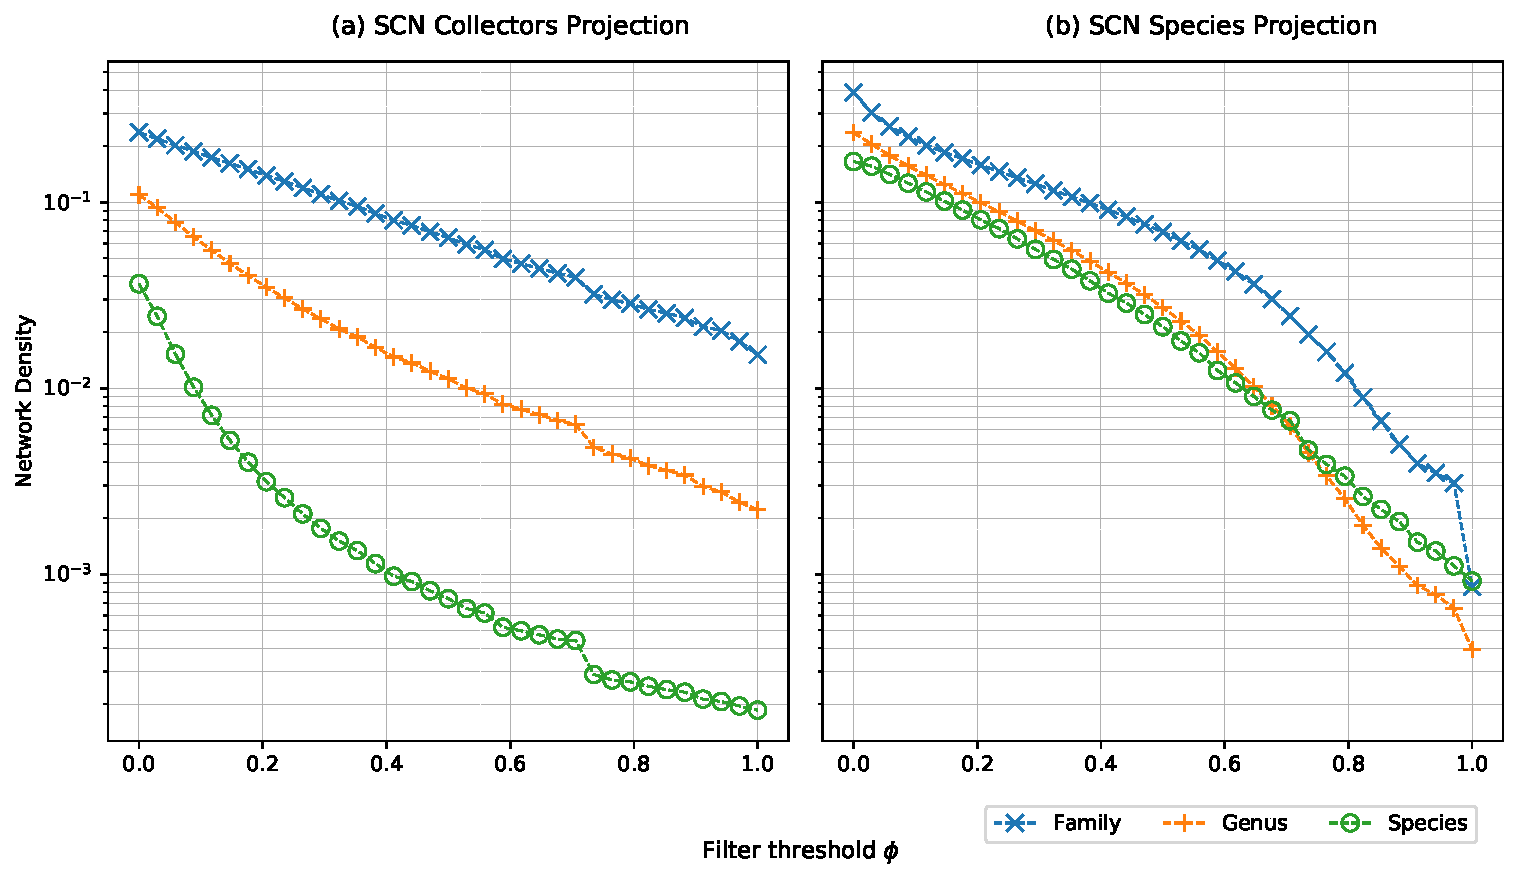
\includegraphics[width=\linewidth]{figures/casestudy_ub/scn_filter_thresh.pdf}
    \caption[Reduction in the density of the species and collectors projections of the UB SCN, as a consequence of increasing filtering threshold.]{ Reduction in the density of the collectors (a) and species (b) projections of the UB SCN, as a consequence of increasing filtering threshold $\phi$. Curves represent the SCN networks aggregated by family (blue), genus (orange) and at the original taxonomic resolution of species (green). }
    \label{fig:ub_scn_filter_thresh}
\end{figure}

In order to investigate the formation of communities in the collectors projection we first filtered collectors ties by setting $\phi = 0.8$.
This means only edges holding similarity scores equal or higher than $0.8$ were kept, while weaker ones were discarded.
This process led to the formation of many small connected components (or \textit{islands}), many of which composed of a single collector.
An additional step in the filtering process was thus required for removing less relevant connected components from the network.
In order to calculate the relevance of a component we defined a simple relevance score which adds up the the values associated to the \textit{count} attribute of each node composing it.
We then removed all islands with score lower than $500$.



% Communities
We applied the \textit{Louvain} heuristic method for community detection \cite{Blondel2008}, which maximizes modularity scores in the network in successive steps.   
The result is an optimized division of the network into modules within which nodes are more densely connected with each other than with external ones.
We also computed the overall taxa composition for each group by summing up the species bags of each of their collectors, which we show as percentages in Table \ref{table:ub_scn_family_projCol_composition}.


\begin{sidewaystable}
\begin{table}[H]
  \caption{Taxa composition for each community as illustrated in Figure \ref{fig:ub_scn_family_projCol_communities}. The total number of distinct taxa, together with the percentages of the top-3 most recorded ones in each community are given.}
  \begin{center}
  \begin{tabular}{r r l l l l}
      community & num of taxa & top taxon & 2nd taxon & 3rd taxon \\
      \hline
0 & 15 & Asteraceae (72.7\%) & Fabaceae (9.1\%) & Melastomataceae (5.2\%) \\
1 & 24 & Cyperaceae (50.4\%) & Fabaceae (9.9\%) & Oxalidaceae (7.2\%) \\
2 & 28 & Fabaceae (58.8\%) & Myrtaceae (8.6\%) & Rubiaceae (6.0\%) \\
3 & 27 & Poaceae (40.4\%) & Cyperaceae (12.5\%) & Asteraceae (7.5\%) \\
4 & 37 & Myrtaceae (62.0\%) & Fabaceae (7.7\%) & Asteraceae (4.3\%) \\
5 & 11 & Rubiaceae (82.7\%) & Myrtaceae (4.6\%) & Fabaceae (3.0\%) \\
6 & 104 & Fabaceae (18.8\%) & Rubiaceae (10.1\%) & Myrtaceae (8.4\%) \\
7 & 27 & Sematophyllaceae (26.8\%) & Hypnaceae (16.0\%) & Dicranaceae (13.8\%) \\
8 & 14 & Desmidiaceae (31.4\%) & Scenedesmaceae (18.9\%) & Chlorellaceae (9.7\%) \\
9 & 23 & Eunotiaceae (35.4\%) & Naviculaceae (15.2\%) & Pinnulariaceae (11.2\%) \\
10 & 2 & Desmidiaceae (97.5\%) & Closteriaceae (2.5\%) \\
11 & 18 & Poaceae (14.3\%) & Fabaceae (13.2\%) & Santalaceae (11.1\%) \\
12 & 4 & Amblystegiaceae (63.6\%) & Polytrichaceae (22.6\%) & Dicranaceae (10.4\%) \\
13 & 5 & Orchidaceae (73.6\%) & Myrtaceae (9.8\%) & Araceae (7.2\%) \\
14 & 9 & Santalaceae (34.5\%) & Loranthaceae (17.4\%) & Myrtaceae (13.4\%) \\
15 & 1 & Melastomataceae (100.0\%) \\
16 & 6 & Fissidentaceae (53.2\%) & Calymperaceae (17.3\%) & Pottiaceae (16.8\%) \\
17 & 7 & Rubiaceae (20.5\%) & Fabaceae (18.8\%) & Dicranaceae (16.2\%) \\
18 & 6 & Arecaceae (36.1\%) & Myrtaceae (25.4\%) & Fabaceae (15.4\%) \\
19 & 4 & Calophyllaceae (38.1\%) & Fabaceae (28.1\%) & Asteraceae (23.8\%) \\
      \hline
  \end{tabular}
  \label{table:ub_scn_family_projCol_composition}
  \end{center}
\end{table}
\end{sidewaystable}


The collectors projection has a total of $20$ communities, $7$ of which are part of the giant component (Figure \ref{fig:ub_scn_family_projCol_communities}). 
Not all collectors from the giant component in Figure \ref{fig:ub_scn_agg_family_general} are also included in the giant component of the collectors-projected SCN.
The biggest community in the giant component is \textit{grp $6$}, including some of the most important UB collectors among which \textit{`irwin,hs'}, \textit{`heringer,ep'}, \textit{`anderson,wr'}, \textit{`ratter,ja'} and \textit{`proenca,ceb'}.
These are generalist collectors, having recorded $104$ from a total of $161$ distinct families, being families \textit{Fabaceae} ($18.8\%$ of the group's interest), \textit{Rubiaceae} ($10.1\%$) and \textit{Myrtaceae} ($8.4\%$) the most recorded ones (Table \ref{table:ub_scn_family_projCol_composition}). 
%
The giant component also includes other smaller communities showing predominant interests towards families \textit{Myrtaceae} (\textit{grp} $4$), \textit{Fabaceae} (\textit{grp} $2$), \textit{Poaceae} (\textit{grp} $3$), \textit{Asteraceae} (\textit{grp} $0$), \textit{Cyperaceae} (\textit{grp} $1$) and \textit{Rubiaceae} (\textit{grp} $5$).

Apart from the giant component there are $7$ other connected components and $6$ isolated nodes, each of them making a distinct community.
The second biggest connected component (\textit{grp{$7$}}) includes part of the bryophytes collectors (polygon $i$ in Figure \ref{fig:ub_scn_agg_family_general}) who are more generalist.
The most recorded family is \textit{Sematophyllaceae} ($26.8\%$), followed by \textit{Hypnaceae} ($16.0\%$) and \textit{Dicranaceae} ($13.8\%$). 
Another part of the bryophytes collectors, who are more specialized towards family \textit{Amblystegiaceae} ($64.6\%$), composes a distinct community (\textit{grp $12$}).
%
Algae collectors from polygon $ii$ (Figure \ref{fig:ub_scn_agg_family_general}) are also split into two distinct communities.
\textit{João Grando} (\textit{grando,jv}) and `\textit{castelobranco,cw}' are placed in \textit{grp~8}, while \textit{leite,alta}' is an isolated node, forming a community of a single collector (\textit{grp $10$}).
\textit{Maria das Graças de Souza} (\textit{souza,mgm}), which is included in polygon $iii$ (Figure \ref{fig:ub_scn_agg_family_general})), is also isolated in the collectors-projected SCN.
The last two collectors mentioned above have very particular taxonomic interests, and are represented as isolated nodes in the projection as they show no strong enough species bags similarities with any other collector in the herbarium.

Although Table \ref{table:ub_scn_family_projCol_composition} gives some intuition on the main taxonomic groups that compose the interests of each community, it is not very informative on how community-specific each of those families are.
Family \textit{Fabaceae}, for instance, has been relatively more recorded by collectors from community $2$ (with $58.8\%$ of the records in that community), although it is also included as a top-3 taxon in communities $0$, $1$, $4$, $5$, $6$, $11$, $17$, $18$ and $19$.
This makes it non-specific, as collectors from many communities have demonstrated interests towards recording it, though to distinct extents.
In contrast, family \textit{Desmidiaceae} is more community-specific, as it is only recorded by algae collectors composing communities $8$ and $10$ (both comprising together only $3$ collectors).
Moreover, it is also relevant to identify groups of families that best split collectors interests in the network by observing which taxa are frequently recorded by common sets of collectors.
A better approach for identifying such groupings of taxa is described below, and consists of changing the projection perspective, focusing on the species set instead.

% ======================
% The Sp set projection
\paragraph{Communities in the species projection.}
\begin{figure}[!ht]
  	\centering
    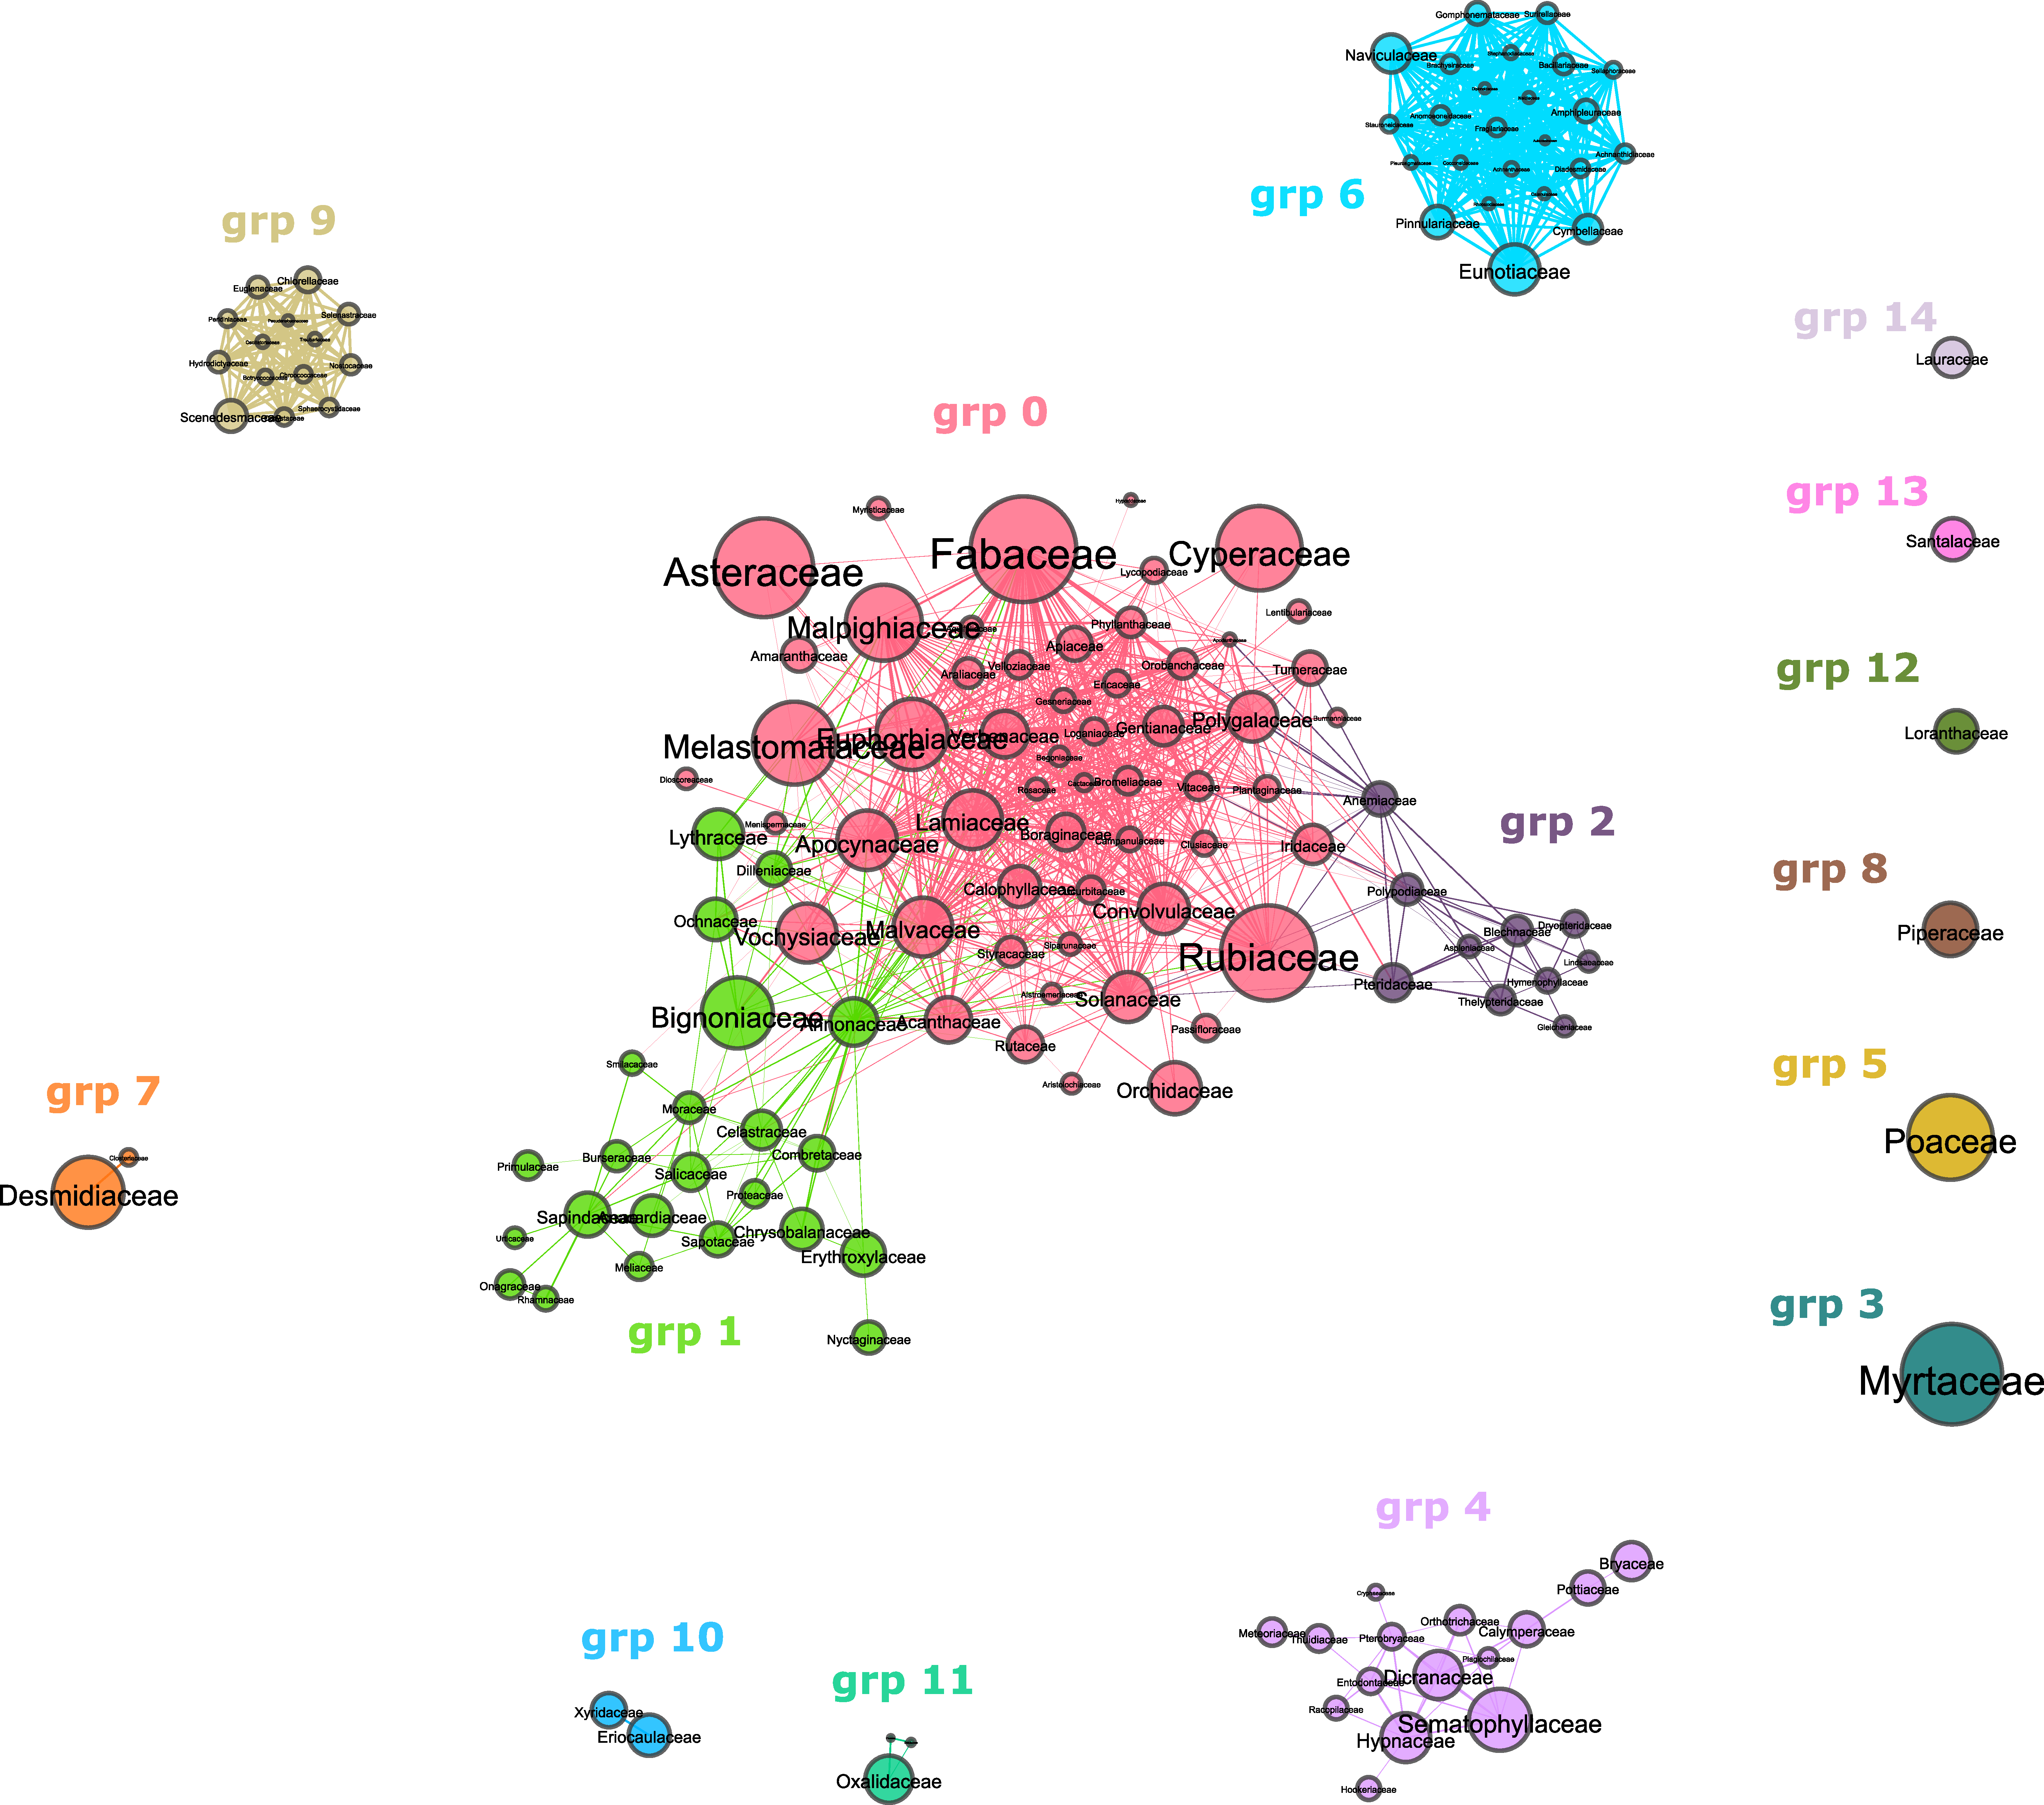
\includegraphics[width=\linewidth]{figures/casestudy_ub/scn_family_projSp_communities.pdf}
    \caption[Communities in the species projection of the family-aggregated SCN.]{ Communities in the species projection of the family-aggregated SCN in figure \ref{fig:ub_scn_agg_family_general}, in which edges with weights lower than $20$ were removed as well as isolated nodes. In order to improve visualization, communities with scores lower than $600$ were also omitted from the figure. Colors are used to distinguish communities and nodes sizes reflect families prevalence in the dataset.}
    \label{fig:ub_scn_family_projSp_communities}
\end{figure}

The species projection of the family-aggregated UB SCN network is a one-mode network exclusively representing taxa at the family resolution, with a total of $474$ nodes, $43756$ edges and average node degree of $184$.
Edges between pairs of taxa are weighted according to their quorum vector similarities, such that strongly connected taxa are those which have been recorded by similar sets of collectors, in similar proportions.
%
The relatively low number of nodes observed in the species projection if compared to the collectors projection stands from the fact that in this case the taxonomic aggregation process does reduce the total number of nodes in the network.
While aggregations at higher taxonomic ranks would result in networks with fewer nodes, network density tends to increase as an effect of the summarization of entities and their ties.
%
It is also important to observe that although the absolute number of nodes and edges in the species-projected network are lower than those from the collectors projection, it is still denser than the latter, with a density score of $3.9 \times 10^{-1}$.

% Filtering
In order to reduce network density and better visualize the formation of communities we performed a filtering routine to remove less relevant families associations, analogously to what we have done for the collectors projection.
As network density decreases with increasing values for $\phi$ (Figure \ref{fig:ub_scn_filter_thresh}b), we again set the threshold value to $0.8$, omitting ties that are weaker than the threshold value. 
As the process produces many islands, we use the same relevance score from the collectors projection for filtering out non-relevant components, though now using a threshold score of $600$. 
This means that islands composed of families whose summed up counts are below $600$ are omitted from the figure. 
The resulting network is shown in Figure \ref{fig:ub_scn_family_projSp_communities}.
Nodes were sized based on the \textit{count} attribute, which indicates how common each family is in the herbarium dataset or, in other words, their \textit{prevalence}. 
Nodes colors reflect the communities they've been assigned to, using the same approach as we did for the collectors projection.

% Communities description
% TODO rephrase
The species projection has a total of $15$ communities, three of which belong to the giant component. 
%
The largest community is \textit{grp $0$}, containing families that are, in general, more widely recorded by herbarium collectors, as it is the case of \textit{Fabaceae}, \textit{Euphorbiaceae} and \textit{Rubiaceae}.
Most of them form a densely-connected structure, containing central families that are all recorded by a very similar set of collectors.
However, there are some families included in the same community which are more loosely connected, and would quickly become isolated nodes if we continued to increase $\phi$. 
This is the case for families \textit{Asteraceae}, \textit{Cyperaceae} and \textit{Orchidaceae}, which indicates that they are recorded by more specialized collectors.
Community $2$, which is also part of the giant component, is exclusively composed of fern families (gymnosperms).
Some of the included families are more recorded by fern specialists, as it is the case of \textit{Gleicheniaceae}, \textit{Dryopteridaceae} and \textit{Hymenophyllaceae}.
Others as \textit{Pterydaceae}, \textit{Anemiaceae} and \textit{Polypodiacea} are recorded by collectors who also record flowering plants such as families \textit{Rubiaceae} and \textit{Iridaceae}.


The remaining $12$ communities are all islands, $6$ of which formed by isolated nodes.
%
Community $4$ contains bryophyte families, mostly recorded by collectors within polygon $i$ in Figure \ref{fig:ub_scn_agg_family_general}.
By observing the low clustering and high diameter of this island, we conclude that bryophyte collectors vary significantly regarding their taxonomic interests, as opposed to what we observe for communities $6$ and $9$, which are very close to being fully connected (cliques).
% Clustered Islands
Community $6$ contains algae families, mostly diatoms (polygon $iii$);
%
while communities $9$ and $7$ are composed by green algae families recorded by collectors within polygon $ii$ in Figure \ref{fig:ub_scn_agg_family_general}.
The reason that nodes from polygon $ii$ give origin to two distinct islands in the SCN species projection is that the taxonomic interests of `\textit{leite,alta}' is substantially distinct from those of `\textit{grando,cw}' and `\textit{castelo-branco,}', and thus families \textit{Desmidiaceae} and \textit{Closteriaceae} are separated from the rest of green algae families.
% isolated nodes
Finally, families \textit{Myrtaceae} (\textit{grp $3$}), \textit{Poaceae} (\textit{grp$5$}) and \textit{Piperaceae} (\textit{grp$8$}) are typically recorded by collectors who are also more specialized in each of those families, and are thus represented as isolated nodes in the network.


% Assortativity in SCN
% Do collectors who have recorded many taxa (generalists) tend to record taxa recorded by many collectors (generalists)? The inverse also holding.

% Network resilience: If the SCN is dissortative, then it is easier to break it by removing hubs (therefore forming many specialized subgroups of collectors). Otherwise, removing any of the main hubs would not have a considerable effect on fractioning the network (Specialized communities are unlikely to be formed if an important collector leaves the herbarium). 


% Conclusion
Communities discussed above are composed of collectors who share interests in common taxa and, conversely, taxa that have been sampled by common sets of collectors.
Collectors with similar interests, however, do not necessarily work together in field, and thus communities of common interests do not correspond to coworking teams.
The latter can be investigated from CWN models instead, which are structured from collaborative ties between collectors.



% ===============================
% UB Collector Coworking Network
% -------------------------------

\subsection{The UB Collector CoWorking Network} \label{section:ub_cwn}
% TODO: Add average path size connecting collectors
% From table \ref{table:ub_collectors_florescer}, \textit{Irwin} mostly contributed to the UB herbarium from year $1962$ to $1976$, in the context of the Central Brazil Expedition carried out by the New York Botanical Garden \footnote{\url{http://sciweb.nybg.org/science2/hcol/planalto/index.asp}}. Together with \textit{William R. Anderson} (\textit{anderson,wr}), \textit{Irwin} was a key member of the expedition staff. 

As the UB CWN was built based on the same set of records as the SCN model explored in the previous section, the number of nodes is $6768$, equivalent to the number of collectors nodes in the SCN model.
A total of $10391$ edges represent collaborative ties between collectors.
The average degree and density for the overall network are, respectively, $3.07$ and $4.5 \times 10^{-4}$.

\paragraph{Connected components.}
The UB CWN is composed of a a total $2991$ connected components, the largest of which --- the giant component ($c_1$) ---  contains $46\%$ of all nodes in the network.
Such a low percentage of nodes in the giant component contrasts to most empirical scientific paper-publishing collaboration networks studied by \citeonline{Newman2001d}, with giant components containing as much as $80\% - 90\%$ of all nodes.
Moreover, only $318$ of the connected components in the UB CWN ($c_1, c_2, ..., c_{318}$) are composed of collectors with at least one collaborative tie.
The remaining $2673$ components ($c_{319}, c_{320}, ..., c_{2991}$) are all disconnected nodes (\textit{i.e.} nodes with $k=0$), which we refer to as \textit{singleton} collectors.

Singleton collectors are those who have never recorded specimens collaboratively --- or at least they have not included the names of their collaborators in the records as authors ---, and thus are considered to have no structural role in the collaboration network.
They comprise $39.5\%$ of all nodes in the network, and the fact that they lack connections impacts on the overall network density, making it relatively low.
In fact, if we instead compute network density by only considering nodes from the giant component $c_1$, we observe an increase in density from $4.5 \times 10^{-4}$ to $1.95 \times 10^{-3}$. 
%
One important example of a singleton collector in the herbarium is `\textit{leite,alta}', with a total of $2757$ records, none of which collaborative (inset in Figure~\ref{fig:ub_team_sizes}).  % of records from all singleton collectors
This comprises $18.14\%$ of all records by singleton collectors.
All other $2672$ singleton collectors have fewer than $400$ records each.
Moreover, $81.1\%$ of occurrences recorded by singleton collectors have been obtained in Brazil.

% Low-degree isolated nodes are probably experienced foreign collectors (who have only contributed to the herbarium with few records (probably exchanges)), as it is unlikely that novice collectors would record alone, without a supervisor. -> Apparently not true


\paragraph{How collaborative are collectors?}
% We use metrics such as average degree, degree distribution, ... as measures of collector collaborativity.

% Team sizes
By inspecting the team sizes of all records in the dataset, we find that the average team size for records in the UB dataset is $1.73$, as a consequence of the fact that $63\%$ of all records are non-collaborative, \textit{i.e.} recorded by a single collector (Figure \ref{fig:ub_team_sizes}).
The number of records as a function of team size seems to decay logarithmically.
\begin{figure}[!ht]
  	\centering
    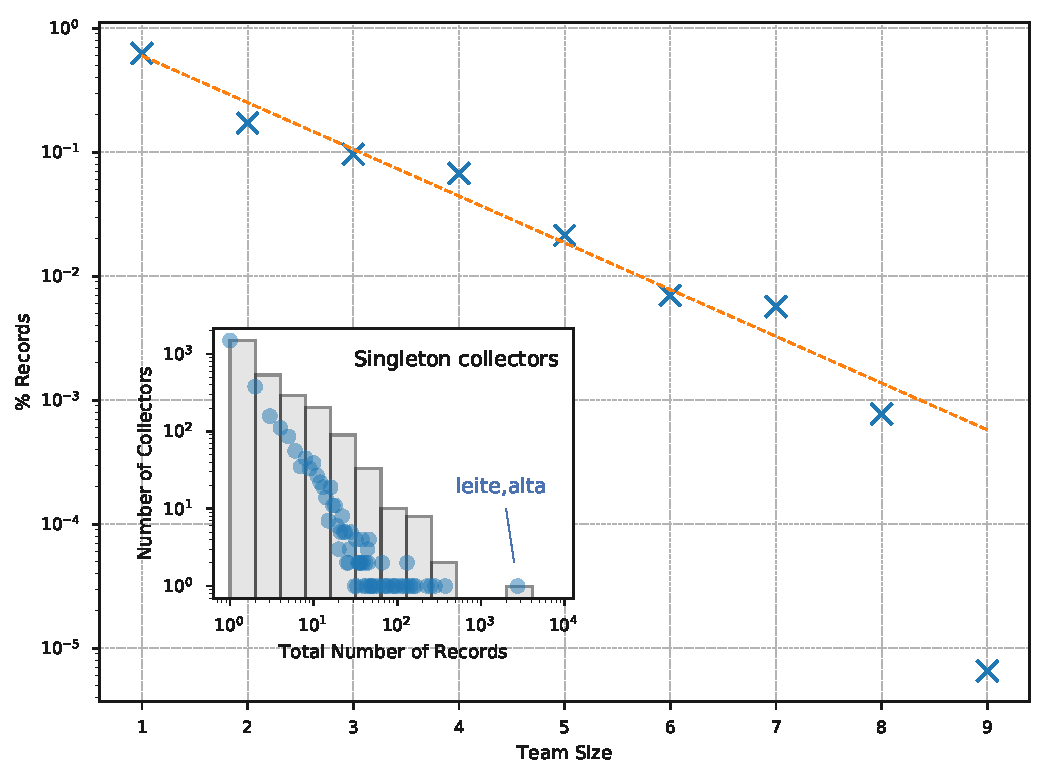
\includegraphics[width=0.9\linewidth]{figures/casestudy_ub/team_sizes.pdf}
    \caption[Percentage of occurrence records in the UB dataset for each team size.]{ Percentage of occurrence records in the UB dataset for each team size. The dashed line represents an exponential fit to the data (using team sizes from $1$ to $8$) using function $f(x) = 10^{\beta_0 + \beta_1 x}$ and parameters $\beta_0=0.16$ and $\beta_1=-0.38$. The inset figure shows the number of records singleton collectors typically hold, with records numbers logarithmically binned using base $2$. }
    \label{fig:ub_team_sizes}
\end{figure}
%
For some reason which is not clear to us, team size is constrained from $1$ to $8$ collectors in this dataset (we consider the single record with team size $9$ to be an artifact).
One hypothesis to be verified is that the data management system adopted by UB imposes limitations on the maximum number of collectors allowed to be registered for each record or, similarly, on the maximum length of the string containing collectors names. 
In fact, we observed that strings containing collectors names are truncated in some records.

Collectors from UB vary substantially regarding their collaborativeness on fieldwork.
Whereas few ones have collaborated with a large number of collectors throughout their careers (much more than the average $3.07$), many of them hold very few collaborative ties.
In fact, almost $40\%$ of them are singleton collectors, having never co-authored a single record.
%
Similarly to the SCN network, the degree distribution of the UB CWN is heavy tailed (Figure \ref{fig:ub_cwn_degree_dist}), and thus is not well fit by a poisson distribution.
Such a topology suggests the existence of non-random processes ruling the probability that two collectors get connected, leading to the co-existence of few hubs and many low-degree collectors.
%% FIGURE: degree dist %%
\begin{figure}[!ht]
  	\centering
    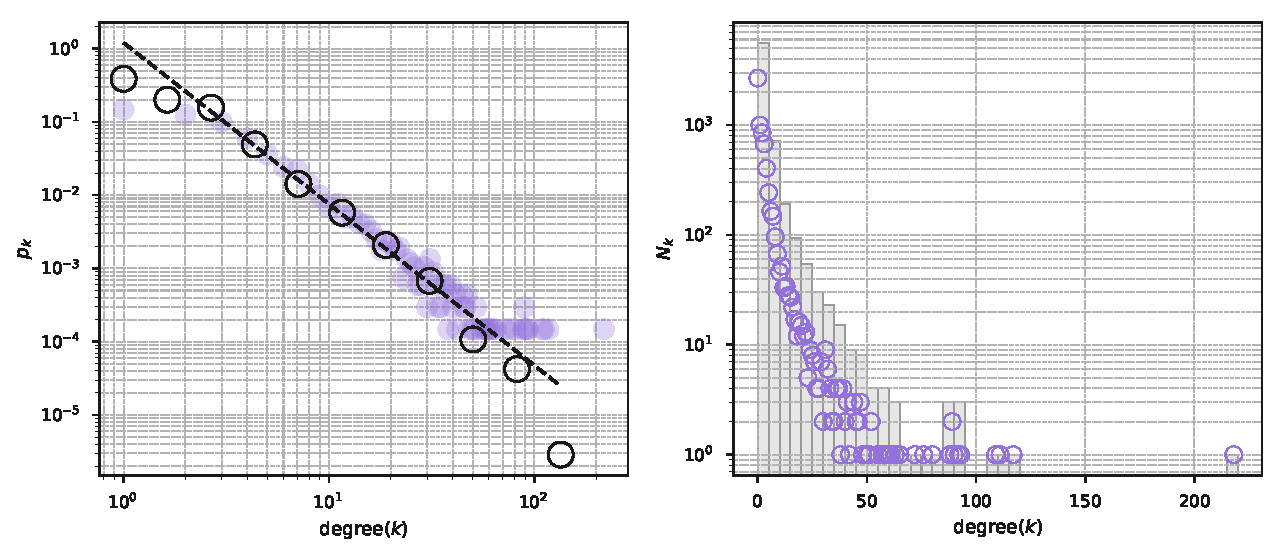
\includegraphics[width=\linewidth]{figures/casestudy_ub/cwn_degree_dist.pdf}
    \caption[Degree distribution for the UB CWN.]{ Degree distribution for the UB herbarium CWN network. Plot (a) shows, using a log-log scale, the probability $p_k$ of finding collectors with each value for $k$. The black line represents a power law function $p(k) \sim k^{-\alpha}$ fit to the data, with $\alpha=2.2$. Purple dots are linearly binned, showing the absolute number of nodes with each degree value. Black circles aggregate degree values by using logarithmic binning. Nodes with $k=0$ were omitted from this plot. Plot (b) shows the absolute number $N_k$ of nodes with each degree (including nodes with $k=0$) in a lin-log scale. The histogram in the background groups nodes degrees in bins of size $5$. }
    \label{fig:ub_cwn_degree_dist}
\end{figure}

Table \ref{table:ub_cwn_degree} ranks the top-20 collectors on weighted degree centrality, using the hyperbolic weighting rule.
As discussed in section \ref{section:cwn}, this rule assigns weights to collectors ties by considering the sizes of the teams in which collectors collaborated, such that higher weights are assigned to ties which were originated from collaborations involving smaller teams (minimum size of $2$).
The weighted degree of a node is given by the sum of the weights of all its edges.
The top collector is `\textit{irwin,hs}', with a weighted degree score of $5696$.
Although he has not collaborated with many distinct collectors (a total of $39$), his position on the rank reflects the absolute number of collaborative records authored by him ($6169$), even though this only comprises $34.1\%$ of all his records. 
%
\begin{table}[t]
  \caption[Top-20 collectors of the UB CWN, ranked by the weighted degree centrality score.]{Top-20 collectors of the UB CWN, ranked by the weighted degree $k_w$ centrality score. Both the absolute number of records and the percentage of those which have been collected collaboratively (involving at least two collectors) are given for each collector. The degree centrality $k$ represents the number of collaborative ties linking a collector to distinct collaborators, whereas the weighted degree is computed with the hyperbolic weighting function.}
  \begin{center}
  \begin{tabular}{l r r r r}
      collector & num of records & \% collaborative & $k$ & $k_w$ \\
      \hline
      irwin,hs & 18065 & 34.1 & 39 & 5696.0 \\
      proenca,ceb & 4803 & 88.3 & 218 & 4203.7 \\
      faria,jeq & 4687 & 82.9 & 117 & 3881.0 \\
      souza,rr & 3885 & 99.3 & 37 & 3835.5 \\
      santos,rrb & 3587 & 94.5 & 41 & 3382.3 \\
      munhoz,cbr & 3191 & 82.8 & 109 & 2493.2 \\
      zanatta,mrv & 2364 & 95.8 & 50 & 2264.0 \\
      castelobranco,cw & 2256 & 100.0 & 1 & 2256.0 \\
      grando,jv & 2256 & 100.0 & 1 & 2256.0 \\
      eiten,g & 3046 & 61.4 & 33 & 1865.5 \\
      amaral,ag & 1825 & 99.5 & 37 & 1815.0 \\
      projetobiodiversidadebp & 1780 & 100.0 & 19 & 1780.0 \\
      mendes,vc & 1696 & 99.9 & 89 & 1695.0 \\
      fonseca,sf & 1610 & 99.9 & 18 & 1607.0 \\
      camara,peas & 2076 & 79.8 & 47 & 1486.0 \\
      harley,rm & 2564 & 66.0 & 90 & 1455.8 \\
      carvalhosilva,m & 1635 & 98.5 & 58 & 1436.0 \\
      eiten,lt & 1262 & 99.6 & 14 & 1256.5 \\
      mello,trb & 1247 & 100.0 & 21 & 1247.0 \\
      soares,aer & 1557 & 73.0 & 29 & 1135.0 \\
      \hline
  \end{tabular}
  \label{table:ub_cwn_degree}
  \end{center}
\end{table}
%
The second collector in the rank, `\textit{proenca,ceb}', has less than a third of \textit{irwin}'s absolute number of records, although $88.3\%$ of them are collaborative. 
With a total of $218$ distinct collaborators, she would be placed at the first position if the rank were built based on the non-weighted degree score ($k$) instead, whilst \textit{'irwin,hs'}, in contrast, would be placed at the $43^{rd}$ position.
%
Another case worth mentioning is that of `\textit{grando,jv}' and `\textit{castelobranco,cw}', both of which have necessarily and exclusively collaborated to each other in all their records (\textit{i.e.}, team size is $2$ for all records).
As a consequence their weighted degree scores $k_w$ are equivalent to the total number of records authored by them ($2256$), whereas their non-weighted degree scores are $k=1$.
%
Thus, the non-weighted degree score $k$ ranks collectors based on their total number of distinct collaborators, irrespective of the  number of times each association has been observed, whilst, on the other hand, the weighted degree score $k_w$ takes into consideration the relevance of each tie, considering that collectors collaborating in smaller teams are relatively more strongly tied.

The \textit{betweeness} centrality metric is also frequently used in social networks analytics for ranking collectors who act as ``bridges'', intermediating a considerable fraction of shortest paths between pairs of nodes in the network. 
We compute betweeness centrality of a node $v$ by making $c_B(v) =\sum_{s,t} \frac{\sigma(s, t|v)}{\sigma(s, t)}$, where $V$ is the node set; $\sigma(s,t)$ is the number of shortest paths between nodes $s, t \in V$ (both $s$ and $v$ different from $v$); and $\sigma(s,t|v)$ is the number of shortest paths between $s$ and $v$ that are pass through $v$ \cite{Brandes2008}. 
The $4$ collectors with highest betweeness centrality scores in the UB CWN are `\textit{proenca,ceb}' ($0.38$), `\textit{faria,jeq}' ($0.18$), `\textit{mendes,vc}' ($0.14$), `\textit{ratter,ja}' ($0.13$).
The first three collectors are also included in the degree centrality rank, in Table \ref{table:ub_cwn_degree}, although `\textit{ratter,ja}' is not (he occupies the $21th$ position, with $k=111$).
By inspecting Figure \ref{fig:ub_cwn_communities}, we verify that in fact all those collectors are in strategic positions.
\textit{Carolyn E. Proença} (\textit{proenca,ceb}) is located at the center of the network, while `\textit{mendes,vc}' and `\textit{faria,jeq}' also interconnect nodes from many distinct communities.
\textit{James A. Ratter} (\textit{ratter,ja}) is a very important node bridging a very relevant group (the green one, around `\textit{irwin,hs}') to the rest of the network.

\begin{figure}[h!]
  	\centering
    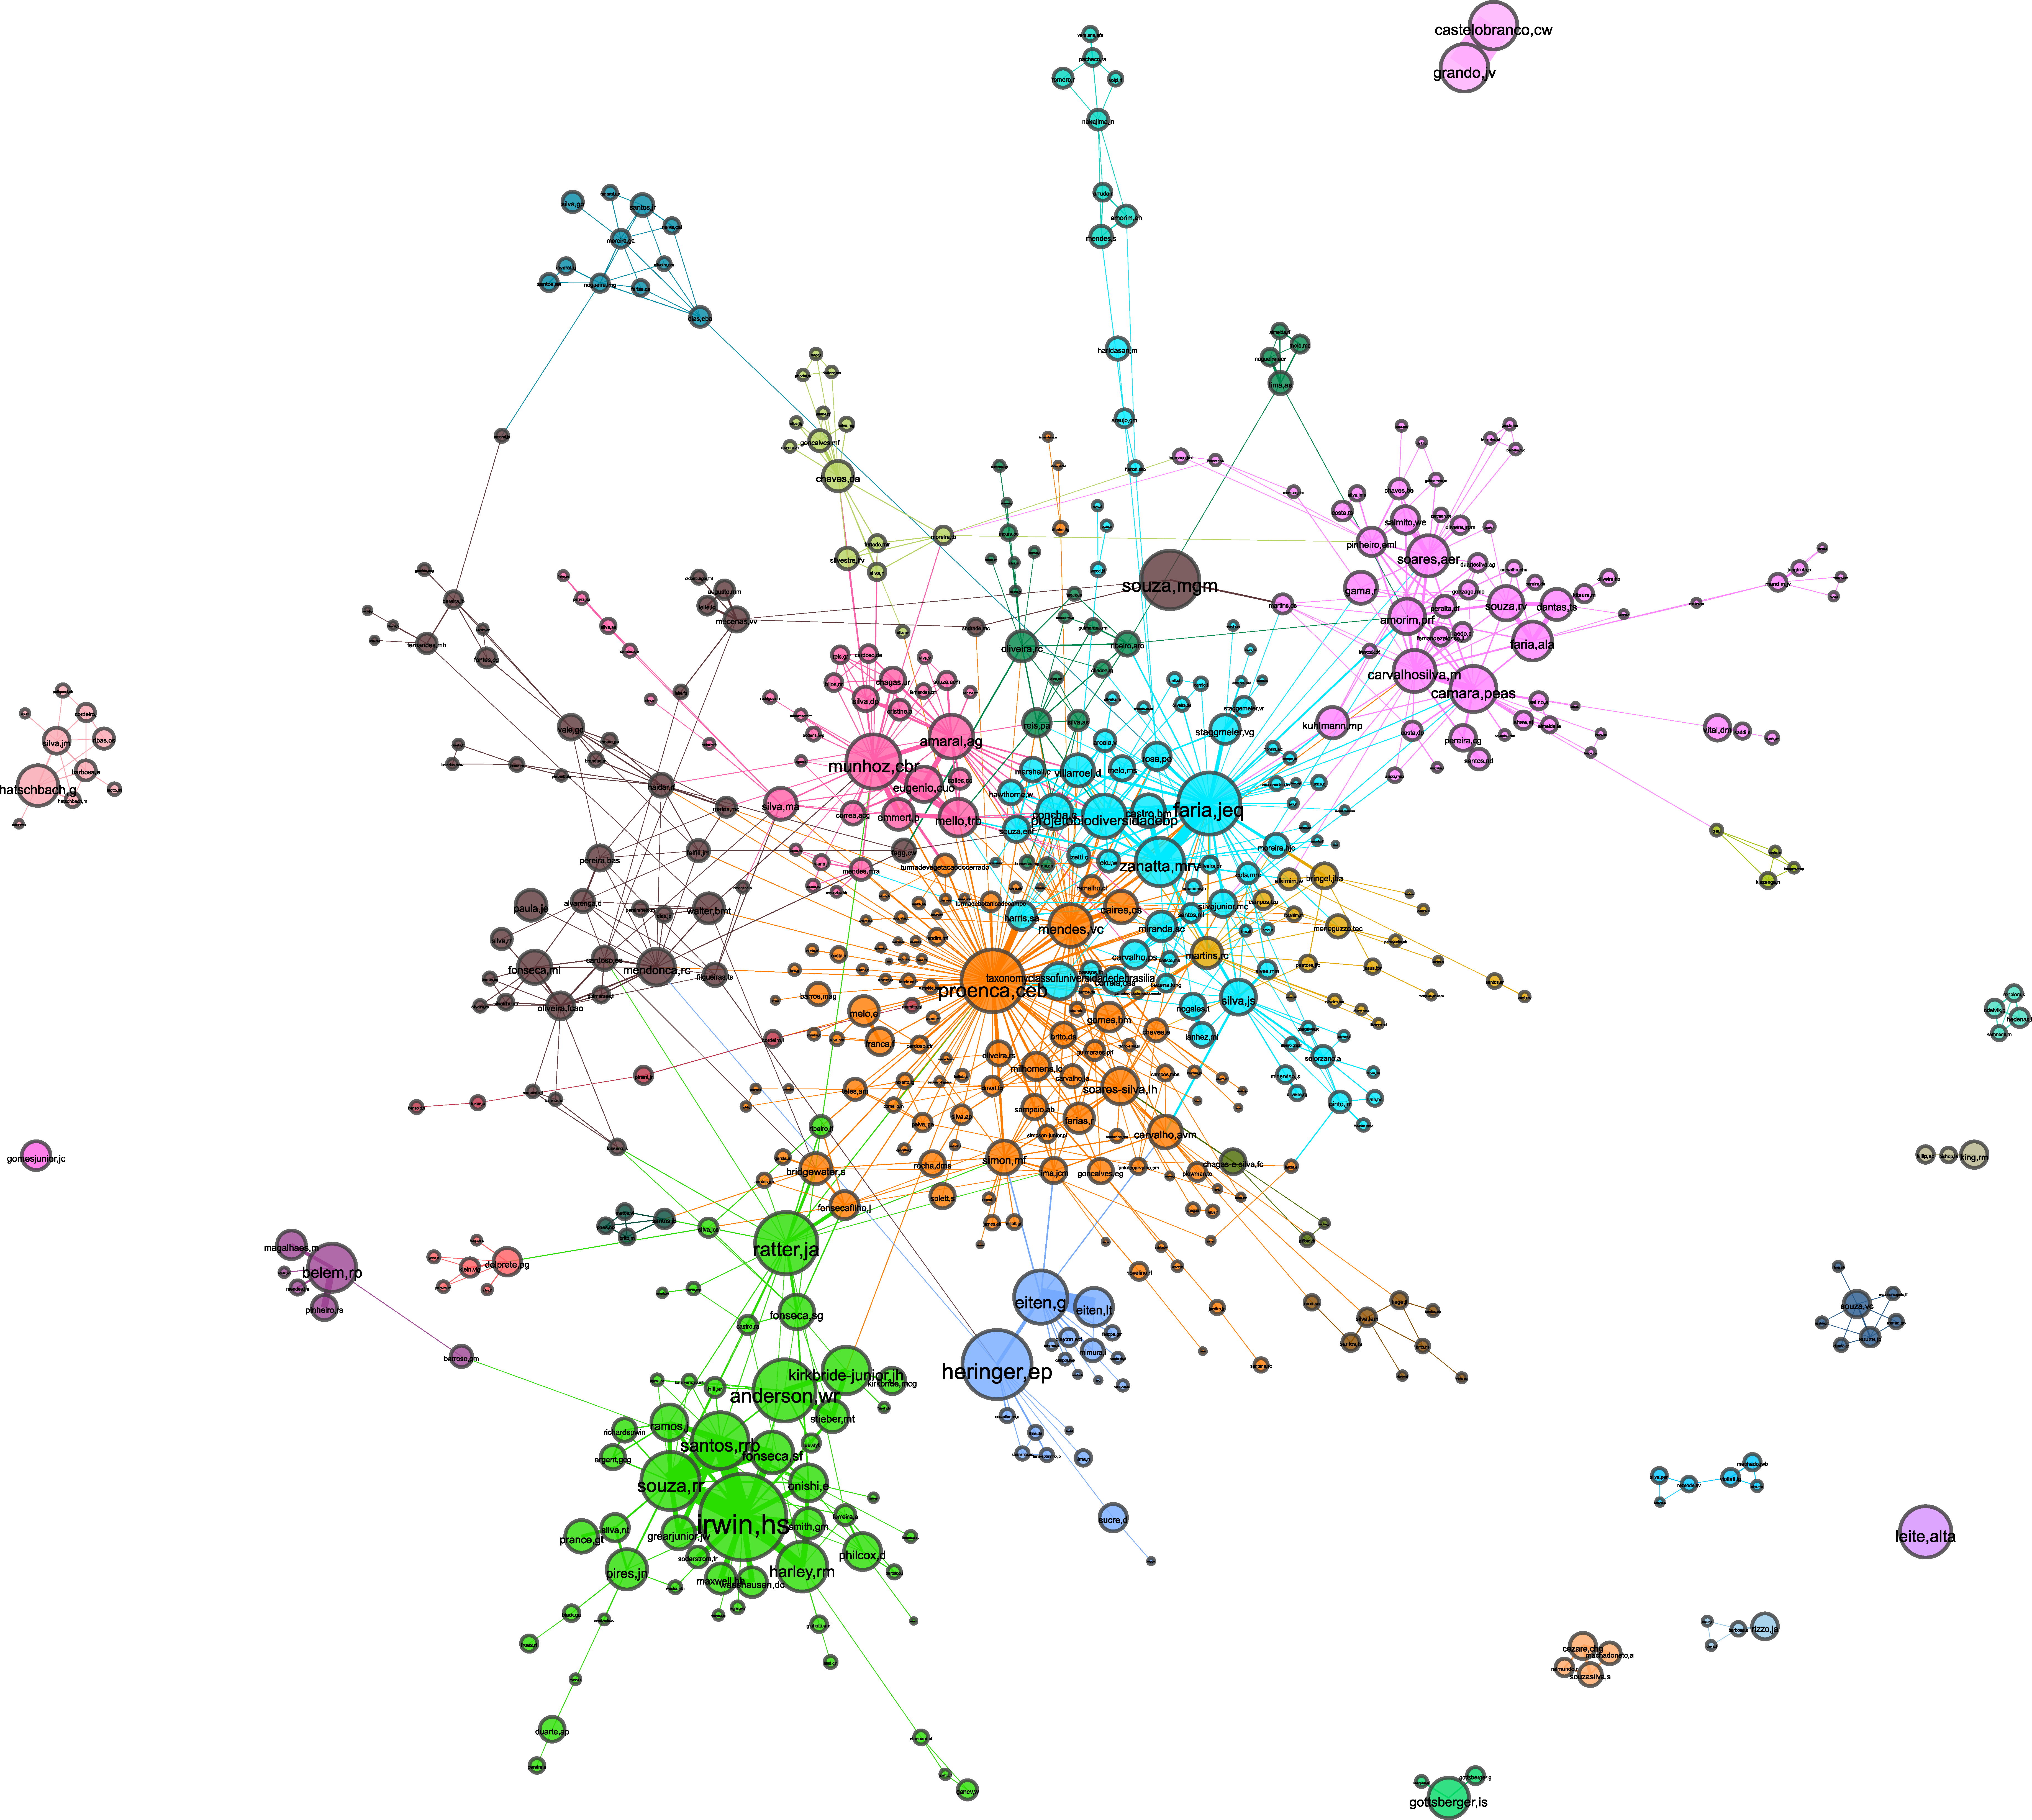
\includegraphics[width=\linewidth]{figures/casestudy_ub/cwn_communities.pdf}
    \caption[Coworking groups in the UB CWN.]{ Coworking groups in a subset of the UB CWN. A total of $30$ distinct communities are differentiated by color. Nodes sizes are proportional to the total number of records of collectors in the dataset. The strength of the ties between each pair of collectors is represented as links thickness.}
    \label{fig:ub_cwn_communities}
\end{figure}


\newpage
\paragraph{Coworking groups.}

One important aspect that can be investigated from the topological structure of the UB CWN is the formation of communities of collectors who co-author specimen records, which we refer to as \textbf{coworking groups}. 
%
In order to detect such groups we have applied the same algorithm for community detection \cite{Blondel2008} as we did for the SCN projections.
%
We detected a total of $30$ distinct communities, $11$ of which are detached from the giant component.
%
For graph visualization, we first performed a filtering routine, similar to that we applied for plotting the SCN projections. 
We first filtered out weaker edges (those with hyperbolic weight lower than $10$), which resulted in many islands. We assigned scores to each island by summing up the values of the \textit{count} attribute of all nodes composing them. 
Islands with scores lower than $600$ were omitted.
The resulting graph has $545$ nodes, $1158$ edges, and average degree of $4.25$ (Figure \ref{fig:ub_cwn_communities}).

% same interest and same coworking
Some of the communities we found in the CWN are formed by collectors who also compose tight communities of interests in the SCN projection (Figure \ref{fig:ub_scn_family_projCol_communities}).
%
One such example is the bryophytes research group, which includes `\textit{camara,peas}', `\textit{carvalhosilva,m}' and `\textit{soares,aer}'.
Collectors from this coworking group (colored in purple and located in the northeast region of the giant component in Figure \ref{fig:ub_cwn_communities}) not only mostly collaborate with members from the same group in field, but are also interested on recording the specific taxonomic group of bryophytes.
%
Another similar example is the coworking group of herbaceous plants collectors (colored in pink), including `\textit{munhoz,cbr}', `\textit{amaral,ag}', `\textit{mello,trb}' and `\textit{eugenio,cuo}', although this group is apparently more open to collaborating with non-members.

% same coworking but distinct interests
Other coworking communities include collectors who happen to be strongly connected with collaborative ties in the CWN despite having distinct taxonomic interests, being weakly connected in the SCN projection.
One such case is that of `\textit{faria,jeq}' and `\textit{zanatta,mrv}', both having recorded a total of $1524$ specimens together (comprising $64.5\%$ of all records by \textit{zanatta,mrv} and $32.5\%$ of all records by \textit{faria,jeq}), and thus belonging to the same coworking group (colored in light blue, Figure \ref{fig:ub_cwn_communities}).
However, as the overall composition of their species bags are substantially distinct (`\textit{faria,jeq}' is more interested on family \textit{Myrtaceae} whereas `\textit{zanatta,mrv}' has a more generalist recording profile), they have been included in distinct interest communities (\textit{grp4} and \textit{grp6}, Figure \ref{fig:ub_scn_family_projCol_communities}).

% same interest but distinct coworking
There are also cases of collectors who, despite having very similar taxonomic interests (being strongly tied in the SCN projection), seldom or never collaborate in field, and are therefore not included in the same coworking groups.
\textit{Daniel Augusto Chaves} (\textit{Chaves,da}) and `\textit{bringel,jba}', for instance, have the majority of their species bags composed of family \textit{Asteraceae} ($54.3\%$ for `\textit{bringel,jba}' and $78.5\%$ for `\textit{chaves,da}'), being both included in the same interest community (\textit{grp0}, Figure \ref{fig:ub_scn_family_projCol_communities}).
However, they have never collaborated on specimens recording, not being adjacent and belonging to distinct communities in the CWN (\ref{fig:ub_cwn_communities}).
%There are apparently no temporal nor geographical impediments explaining the fact that they have never recorded together, as both have a considerable amount of records in the states of Goiás and Minas Gerais and have contemporary careers, with peaks of recording activity around $2011-12$ for \textit{bringel,jba} and around $2013-14$ for \textit{chaves,da}.
%
For another example, the community around `\textit{hatschbach,g}' (at the leftmost region of the figure) is an island in the CWN, as it incorporates no relevant collaborations with collectors from the giant component.
However, given their taxonomic interests at the \textit{family} rank, members of that community are included in the giant component of the SCN (\textit{grp$6$}).


% why communities of interest do not overlap with coworking communities
We consider some possible explanations for why groups of collectors with very similar taxonomic interests would not also form collecting coworking teams.
%
First, as coworking relations are based on the physical recording of organisms taking place at some location and date, they can only possibly exist between collectors whose recording activities overlap both in geographical and temporal spaces.
As temporal and geographical distances between collectors increase, they consequently become more unlikely of developing collaborations, constrained by the limited lifespan of their own careers.

Second, non-professional relationships could also facilitate or hinder the establishment of new coworking ties between individuals. 
Positive relationships (\textit{e.g.} friendship) could lead two collectors to collaborate irrespective of their own taxonomic interests, for instance, if they simply mean to be companions of each other and help their friend on field collections.
On the other hand negative relationships, such as rivality, can prevent potentially fruitfull coworking relationships to establish between collectors who record very similar taxonomic groups at the same place and time.
Moreover, people have limited information on the activities of other collectors and research groups, and thus might not collaborate simply as a consequence of not being acquainted of each other.

Last, we might fail to grasp a complete picture of how interest groups are truly structured in the SCN depending on the taxonomic resolution we adopt while inspecting it.
To exemplify, consider the scenario in which we detect a subset of collectors composing a community in a family-aggregated projected SCN, such as that in Figure \ref{fig:ub_cwn_communities}.
At the taxonomic resolution of family, we would naturally assume that all those collectors have very similar taxonomic interests, as the reason they are included in the same community is that they have very simlar ``families signatures'' distinguishing them from the rest of the collectors. 
However, if we increased the taxonomic resolution of the model (\textit{e.g.} to genus), we might observe the community to subdivide, each of them containing collectors who, although interested in the same family, collect distinct sets of organisms belonging to it.
Subcommunities that emerge in higher-taxonomic resolution SCNs are thus not detectable in lower-resolution aggregations.


% Temoral evolution of the CWN
\paragraph{Temporal evolution of the CWN.}
Finally, we investigated the temporal evolution of communities in the UB CWN by rendering a sequence of frames covering the period from $1955$ to $2017$, each spanning a period of $7$ years (Figure \ref{fig:ub_cwn_temporal_evol}).
Frames aggregate and display collaborations (edges) occurring within the respective periods, and only collectors showing significant activity within each period are plotted.
We consider the activity of a collector to be significant if the number of occurrences recorded within the period comprises at least $5\%$ of his/her absolute number of records.
Although our proposed CWN model does not incorporate the temporal dimension in its structure, we were able to build the frames by querying the UB species occurrence dataset from which the network was constructed.

\begin{figure}[h!]
  	\centering
    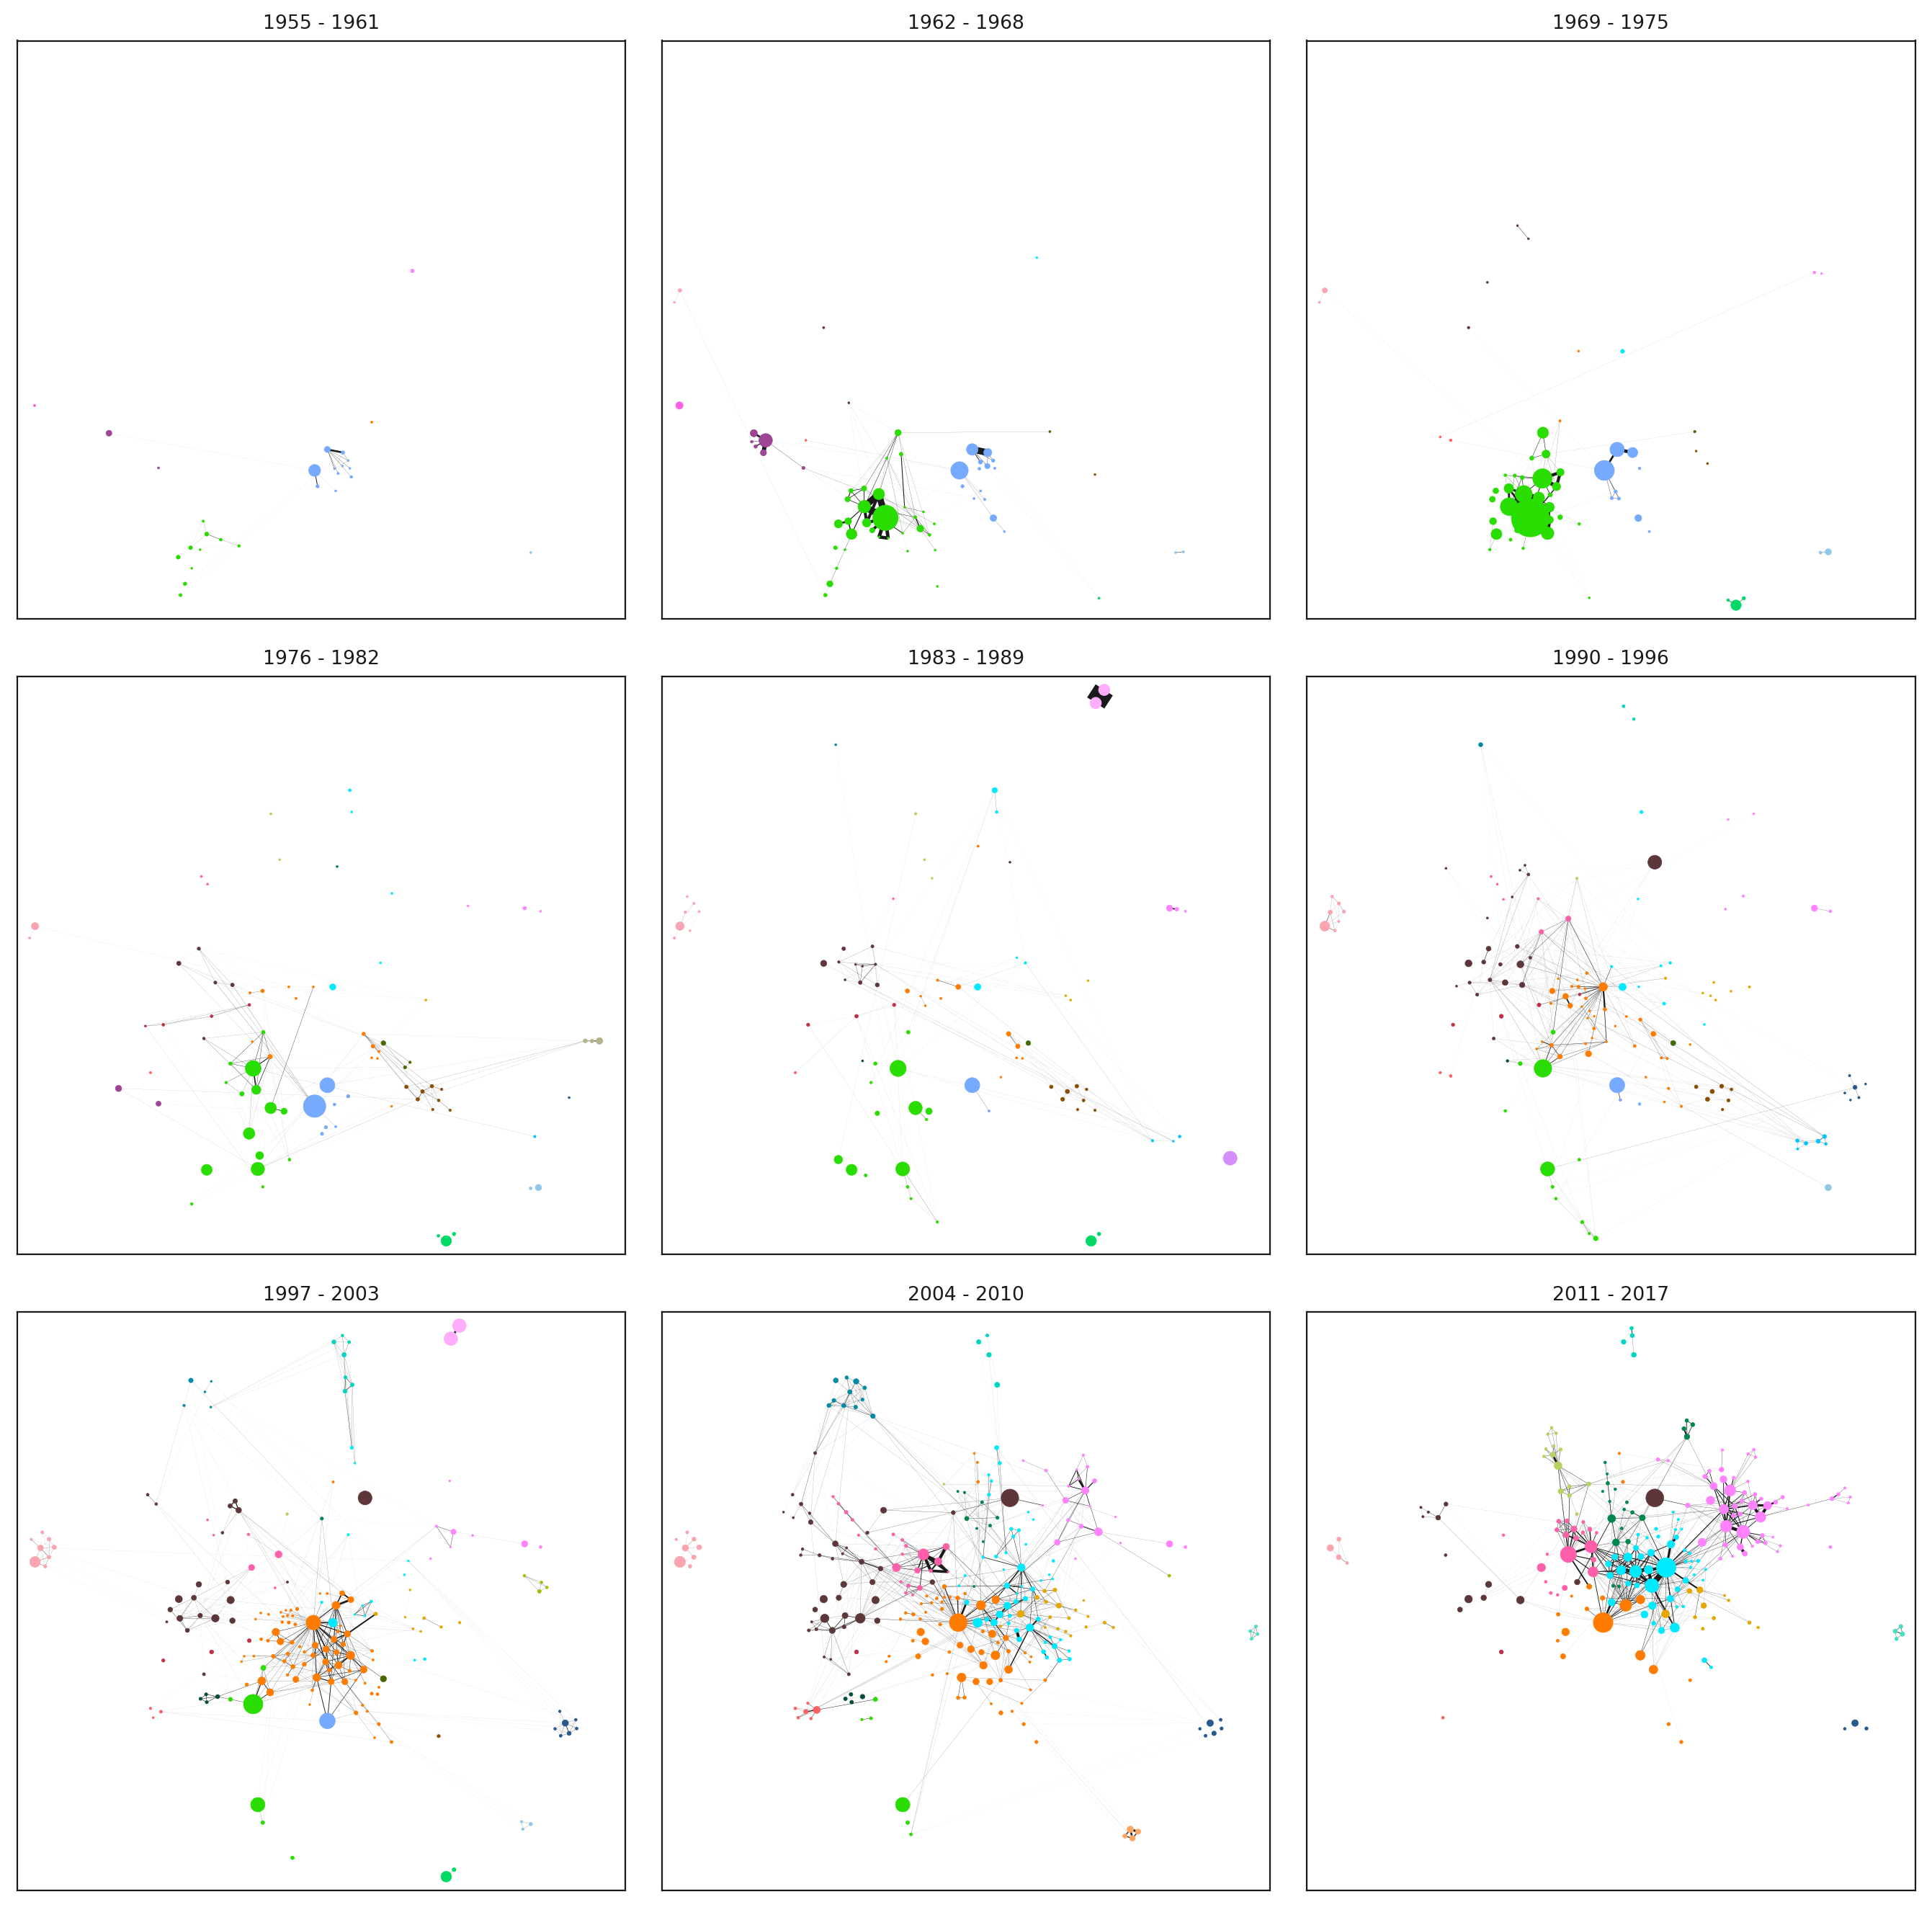
\includegraphics[width=\linewidth]{figures/casestudy_ub/cwn_temporal_evol.png}
    \caption[Temporal evolution of the UB CWN.]{ Temporal evolution of the CWN shown in Figure \ref{fig:ub_cwn_communities}. Each frame corresponds to a period of $7$ years, and only collectors with significant activities in the respective periods are drawn in each frame. Nodes sizes are proportional to the total number of records of each collector up to the end of each period; and the thickness of ties are proportional to how intensively collectors have collaborated during each period (using the hyperbolic weighting rule). The layout of nodes in the figure is the same as from Figure \ref{fig:ub_cwn_communities}. }
    \label{fig:ub_cwn_temporal_evol}
\end{figure}

Three pioneer collectors groups, which we refer to as the \textbf{first generation} of botanists (with most of their recording activities concentrated from $1955$ to $1982$), were historically remarkable for having largely contributed to the early formation of the UB herbarium (frames $1-4$ in Figure \ref{fig:ub_cwn_temporal_evol}).
% First generation (1955-82)
% Blue group
The first group (colored in blue-gray) includes `\textit{heringer,ep}', `\textit{eiten,g}' and `\textit{eiten,lt}'.
\textit{Ezechias Paulo Heringer} (\textit{heringer,ep}) is regarded as one of the founders of the UB herbarium, having led the first exploratory expeditions for sampling the flora of the Federal District \cite{Walter2001}.
During his earlier activities (around $1955$) he has collaborated with `\textit{castellanos,a}', a renowned Argentine botanist who visited the region during the construction of the city of Brasília.
Later in his career ($1969$ to $1975$), `\textit{heringer,ep}' has also teamed up with `\textit{eiten,g}', recording specimens mainly in the states of Minas Gerais and Goiás.
\textit{George Eiten} (\textit{eiten,g}) is also considered a historically relevant collector for the herbarium, having contributed with an extensive set of plant records, mainly from the Cerrado biome \cite{Gomes2012}.
\textit{Eiten}'s known strong collaboration with first his first wife, `\textit{eiten,lt}', is captured by our network model, as shown in the first $3$ frames in Figure \ref{fig:ub_cwn_temporal_evol}.

% Green group
A second group which also heavily contributed to the formation of the herbarium is the one composed by `\textit{irwin,hs}', `\textit{anderson,wr}', `\textit{ratter,ja}', `\textit{harley,rm}', `\textit{pires,jn}', among others (colored in green).
\textit{Howard Irwin} (\textit{irwin,hs}) was the head of a series of exploratory expeditions to the Central Brazilian Highlands from $1964$ to $1971$, which were part of a collaborative program between the New York Botanical Garden (NYBG) and the University of Brasília \cite{Irwin1996}.
Since the beginning of the of the expeditions we observe a strong association between \textit{irwin,hs} and two of his field assistants (\textit{souza,rr} and \textit{santos,rrb}), shown in frames $2$ and $3$ from Figure \ref{fig:ub_cwn_temporal_evol}.
Other important collectors, including `\textit{harley,rm}', `\textit{fonseca,sf}' and `\textit{onishi,e}', have later on joined the team around `\textit{irwin,hs}', contributing to the expedition in the period from $1969$ to $1975$.
%
It is also noticeable the association between `\textit{anderson,wr}', `\textit{kirkbride-junior,jh}' and `\textit{stieber,mt}', in the time frame from $1969$ to $1975$.
\textit{William Anderson} (\textit{anderson,wr}) was a botanist from the NYBG, who continued the expeditions initiated by his colleague `\textit{irwin,hs}' on $1971$ \cite{Irwin1996}, together with `\textit{kirkbride-junior,jh}', a graduate student at the same institution.
%
\textit{James Ratter} (\textit{ratter,ja}) was another important collector of the herbarium, having collaborated with at least two different generations of botanists.
We therefore consider him to be a ``temporal bridge'', connecting two important parts of the network which do not overlap temporally.
\textit{George Eiten} (\textit{eiten,g}) has also collaborated with second-generation collectors (\textit{simon,mf}, \textit{lima,cjm} and \textit{carvalho,avm}) within a period from $1997$ to $2003$, after at least $21$ years with no recording activities.
%
% Purple group
The third group (colored in purple) is smaller, composed of $6$ collectors including \textit{magalhaes,m} and \textit{belem,rp}, the latter a brazilian student who has mostly collected at the state of Bahia from $1955$ to $1968$.

% Second generation (1983-2003)
The \textbf{second generation} of collectors are those more active within the period from $1983$ to $2003$ (frames $5$ to $7$), and are placed more towards the central region of the network.
%
Two relevant collectors from the earlier second generation are `\textit{castelobranco,cw}', `\textit{grando,jv}' and `\textit{leite,alta}', all algae collectors with most of their activity ranging from $1983$ to $1989$.
As we previously pointed out in this text, `\textit{castelobranco,cw}' and `\textit{grando,jv}' have collaborated on all their records, whereas `\textit{leite,alta}' is a singleton collector, having no collaborative records at all. Other important second-generation collectors are `\textit{proenca,ceb}' and `\textit{souza,mgm}', with most intensive activities concentrated from $1990$ to $2003$.
Whereas `\textit{souza,mgm}' has almost exclusively collected within the period from $1990$ to $1996$ and with very few collaborations, `\textit{proenca,ceb}' has extended has extended her collecting activities until current date ($2017$), having collaborated with a very high number of collectors, including the first-generation collector `\textit{ratter,ja}'.
\textit{Cássia Munhoz} (\textit{munhoz,cbr}) starts her activities around $1990$, being one of the founders of a coworking community around herbaceous plants.

% Third generation (2004-2017)
Finally, we assign collectors whose activities are concentrated from $2004$ to $2017$ to the \textbf{third generation}, the most prominent one being `\textit{faria,jeq}'.
As shown in the graph, `\textit{faria,jeq}' has intensively collaborated with important collectors from distinct coworking communities, including `\textit{zanatta,mrv}', `\textit{staggmeier,vg}', `\textit{amorim,prf}', `\textit{proenca,ceb}', `\textit{amaral,ag}', `\textit{bringel,jba}' and `\textit{ribeiro,aro}', mainly in the period from $2011$ to $2017$.
%
Other important collectors from this generation are `\textit{amaral,ag}', `\textit{eugenio,cuo}' and `\textit{mello,trb}', having collaborated more intensely from $2004$ to $2010$. They form a community around the second-generation collector `\textit{munhoz,cbr}', who was also their academic advisor during graduate research.
%
% pink group
An important community which emerged during this period is the bryophytes lab team. 
\textit{Paulo Eduardo Câmara} (\textit{camara,peas}) initiated his recording activities in $1997-2003$, followed by `\textit{carvalhosilva,m}' and `\textit{soares,aer}' in $2004-2010$. These three collectors formed the base of the group, which grew significantly in the period from $2011$ to $2017$, as it was joined by several students. 



% TODO: Betweeness: Which collectors facilitate collaborative behavior?
 
 



%%% QUESTIONS

%% 1. How common are collaborative recordings within the dataset?
%%% What is the proportion of collaborative records in the dataset? How many collaborators
%%% One-collector recording vs >2 collectors recordings
%%% Distribution of team size
%%% Caveats: Some collectors may not include collaborators names in the records

%% x. How likely is a novice collector to become a great collector?

%% x. Do collectors with similar interests tend to collect together?
%%% Mix of the two models
%%% Look for homophily in collectors communities, assortativity.

%% x. Which groups of species best partitionate collectors in the dataset, in terms of their collection interests? 
%%% Using SCNs
%%% Are these groups necessarily taxonomic ones (such as family)? Or could functional groups be more relevant in some cases? Or is there a geographical effect?
%%% e.g. Some group might be best classified as specialists on species inhabiting some geographical location, with some specific habit and belonging to some family rather than simply as specialists in a given family.

%% x. The Expert-location problem {Chapt. 8 of book Social Network Data Analytics}
%%% The expert team formation problem: How can we best select experts for a given job, based on how willing they are of collaborating together?
%%% Combine both SCN and CWN


% Statistical characterization of CWN structure
%% Largest component, connected components...
%% Assortativity: Do collectors with many collaborators (very collaborative) tend to associate with others that are also very collaborative?






%\subsection{Features Selection}

%% Features engineering

%\section{Model Evaluation}

